%% POSIM - IPM Journal Submission
\documentclass[a4paper,fleqn]{cas-dc}

\usepackage[authoryear,longnamesfirst]{natbib}
\usepackage{amsmath}
\usepackage{algorithm}
\usepackage{algorithmic}
\usepackage{array}
\usepackage{graphicx}
\usepackage{booktabs}
\usepackage{multirow}
\usepackage{colortbl}
\usepackage{xcolor}
\usepackage{makecell}
\usepackage[most]{tcolorbox}
\usepackage{subfig}
\usepackage{wrapfig}
\usepackage{fontspec}
\setmainfont{Times New Roman}
\setsansfont{Arial}
\setmonofont{Courier New}
\ExplSyntaxOn
\cs_if_exist:cT { not= } { \cs_undefine:c { not= } }
\cs_if_exist:cT { not< } { \cs_undefine:c { not< } }
\cs_if_exist:cT { not> } { \cs_undefine:c { not> } }
\ExplSyntaxOff
\usepackage{unicode-math}
\setmathfont{XITS Math}

\usepackage{xeCJK}
\setCJKmainfont[BoldFont=SimHei,ItalicFont=KaiTi]{SimSun}
\setCJKsansfont{Microsoft YaHei}
\setCJKmonofont{FangSong}

\usepackage{listings}
\lstset{
  basicstyle=\scriptsize\ttfamily,
  breaklines=true,
  frame=none,
  columns=fullflexible,
  keepspaces=true,
  aboveskip=2pt,
  belowskip=2pt,
}
\usepackage{enumitem}
\usepackage{etoolbox}
\usepackage{placeins}
\AtBeginEnvironment{tabular}{\fontspec{Times New Roman}}

\renewcommand{\footnotesize}{\scriptsize}

\usepackage{caption}
\captionsetup{font={small,rm},labelfont={bf},labelsep=newline}
\captionsetup[table]{font={small,rm},labelfont={bf},labelsep=newline}
\captionsetup[figure]{font={small,rm},labelfont={bf},labelsep=newline}

\hypersetup{citecolor={blue!80!black},linkcolor={blue!80!black},urlcolor={blue!80!black}}
\graphicspath{{figures/}}

\definecolor{oursrow}{RGB}{232,245,233}
\definecolor{greenrow}{RGB}{228,245,228}
\definecolor{orangerow}{RGB}{255,245,230}
\definecolor{purplerow}{RGB}{245,240,255}
\definecolor{grayrow}{RGB}{240,240,240}
\definecolor{promptbg}{RGB}{242,247,253}
\definecolor{promptborder}{RGB}{70,130,180}
\definecolor{gaingreen}{RGB}{34,139,34}

\newtcolorbox{promptbox}{
 colback=promptbg, colframe=promptborder,
 boxrule=0.5pt, arc=1mm,
 left=4pt, right=4pt, top=4pt, bottom=4pt,
 breakable, enhanced}

\newcommand{\best}[1]{\textbf{#1}}
\newcommand{\na}{\text{---}}
\newcommand{\posim}{\textsc{Posim}}
\newcommand{\gain}[1]{{\textcolor{gaingreen}{\,#1}}}

\def\tsc#1{\csdef{#1}{\textsc{\lowercase{#1}}\xspace}}
\tsc{WGM}
\tsc{QE}

\begin{document}
\let\WriteBookmarks\relax
\def\floatpagepagefraction{1}
\def\textpagefraction{.001}

\shorttitle{POSIM：面向社交媒体舆情演化的多智能体仿真框架}
\shortauthors{Y. Zhang et al.}

\title [mode = title]{POSIM: A Multi-Agent Simulation Framework for Social Media Public Opinion Evolution}

\author{Yongmao Zhang}
\credit{Conceptualization, Methodology, Software, Writing - Original draft}

\author{Kai Qiao}

\author{Zhengyan Wang}

\author{Wenyao Sun}

\author{Dekui Ma}

\author{Ningning Liang}

\author{Jian Chen}

\author{Bin Yan}
\cormark[1]

\affiliation{organization={Henan Key Laboratory of Imaging and Intelligent Processing, Information Engineering University},
            city={Zhengzhou},
            postcode={450001},
            country={PR China}}

\cortext[1]{Corresponding author}
\fntext[1]{These authors contributed equally to this work.}

\begin{abstract}
解析并预判社交媒体舆情的演化过程，对于社会治理具有重要意义。然而，传统舆情建模方法，如传染病模型和基于规则的智能体模型（ABM），难以刻画真实社交用户的复杂认知过程和环境适应能力。近年来兴起的基于大语言模型（LLM）的社会模拟技术，虽已用于分析极化、从众和信息传播等特定群体现象，但仍难以再现真实社交媒体舆情中非理性的个体交互和多阶段的演化过程。
本文提出 POSIM（\textbf{P}ublic \textbf{O}pinion \textbf{Sim}ulator），一个面向社交媒体舆情演化的多智能体仿真框架。POSIM 首先构建受信念-欲望-意图（BDI）理论启发设计的 LLM 智能体来模拟非理性社交用户，然后搭建了包含社交网络和曝光机制的虚拟社交媒体环境，最后引入基于点过程的时间动力学引擎，以统一刻画智能体与环境持续耦合下的舆情多阶段演化过程。
为系统检验框架的可信性，我们基于微博平台构建了覆盖原帖、转发与评论全链路交互的真实舆情数据集，实验表明，POSIM 成功复现了真实舆情在个体交互机制与群体现象涌现上的关键特征，并在多个舆情指标上验证了框架的有效性。进一步地，我们基于 POSIM 开展治理导向的策略干预实验，发现共情式引导在特定条件下反而加剧了舆论负面情绪这一反直觉的“共情悖论”现象。上述结果表明，POSIM 可作为计算实验平台支持有效的事前策略推演，为舆情治理提供可量化的决策依据。
\end{abstract}

% \begin{highlights}
% \item 提出Social-BDI元认知智能体架构，将大语言模型嵌入分层认知框架实现具有可追溯决策链的舆情行为仿真
% \item 基于霍克斯自激点过程构建时间-事件混合驱动仿真环境，支持分钟级时间分辨率的长周期连续仿真
% \item 建立三层递进验证体系，在三个真实微博数据集上行为、内容和拓扑层面全面优于基线方法
% \item 高度解耦的模块化架构保证各组件独立替换与功能扩展，案例研究验证了框架在舆情治理场景中的应用价值
% \end{highlights}

\begin{keywords}
社交媒体仿真 \sep 舆情分析 \sep 大语言模型 \sep 智能体认知架构 \sep 霍克斯过程
\end{keywords}

\maketitle

% ============================================================
% 第1节 引言
% ============================================================
\section{引言}\label{sec:intro}

社交媒体已成为公共舆论形成、发酵与扩散的关键场域，一则突发事件往往能在数小时内引发大规模用户参与，并伴随复杂的群体情绪唤醒过程~\citep{gonzalez_emotional_2010}和信息级联~\citep{goldstein_structure_2012}。理解并预判舆情演化过程，对社会治理具有重要意义~\citep{WU2025127823}。然而，真实世界中的社会实验通常受限于伦理约束、不可重复性与变量不可控等根本困难，难以直接在现实场景中反复检验不同机制与干预方案。因此，计算仿真成为研究舆情演化规律、开展策略推演并支撑治理决策的重要技术路径~\citep{bonabeau_agent-based_2002}。

要构建能够复刻真实舆情演化的仿真系统并不容易。一方面，社交媒体用户的行为并非简单理性决策，而是受个体和环境的多因素交互影响驱动~\citep{buckels2014trolls}，系统需要刻画这一复杂的认知决策过程；另一方面，舆情演化具有显著的时变特征，事件往往在短时间内集中爆发，并经历爆发、回落、复燃等多阶段演化~\citep{ZHOU2024121307}，这对仿真的时间动力学精度提出了更高要求~\citep{zhao_seismic_2015}。此外，仿真系统还必须回答“结果为何可信”这一关键问题：不仅要在外部结果层面与真实数据相接近，还要说明其内部演化机制是否合理可信~\citep{mcculloch_calibrating_2022}。传统舆情建模方法如传染病模型~\citep{daley_stochastic_1965}和阈值级联模型~\citep{granovetter_threshold_1978}，通常将个体简化为少量离散状态，难以表达复杂语义、互动策略与用户异质性；基于智能体的建模（ABM）虽提供了自下而上的仿真范式~\citep{macal_tutorial_2010}，并常结合观点动力学规则刻画群体演化~\citep{castellano_statistical_2009}，但规则驱动的智能体仍难以刻画真实用户的认知决策、复杂互动及其与平台环境之间的耦合过程。

近年来，大语言模型（LLM）驱动的社会仿真为这一领域带来了新的转机~\citep{wang_survey_2024}。以生成式智能体建模（Generative Agent-Based Modeling, GABM）~\citep{park_generative_2023}为代表的研究表明，LLM智能体已能够生成类人的社交行为，并在多智能体交互中成功涌现出极化、从众、信息扩散等复杂社会现象~\citep{gao_s3_2023,chuang_simulating_2024}。然而，要建模更为复杂的真实舆情演化过程，仍需进一步刻画真实用户受认知信念驱动的非理性特征，并在短时间内捕捉舆情从环境事件触发、用户响应再到传播放大的协同演化过程。因此，当前仍缺少一个既面向真实舆情演化、又具备结果可信性的统一仿真框架。

基于这一背景，本文提出POSIM（\textbf{P}ublic \textbf{O}pinion \textbf{Sim}ulator），一个面向真实社交媒体舆情演化的多智能体仿真框架。框架首先构建受信念-欲望-意图（BDI）认知理论~\citep{bratman_intention_1987,rao_bdi_1995}启发的LLM智能体，将情绪唤醒与认知偏差等非理性因素融入分层认知架构，使其具备显式的认知状态与可追溯的多阶段决策链路；然后搭建包含社交网络与信息曝光机制的虚拟社交媒体环境；最后引入基于霍克斯点过程的时间动力学引擎~\citep{hawkes_spectra_1971}，统一刻画外生事件冲击与内生用户交互共同驱动下的舆情多阶段演化过程。

为避免仿真评估陷入“结果看似吻合、机制却无法解释”的虚假繁荣，本文进一步从“机制-现象-数据”三个层次对仿真系统的可信性进行完备验证~\citep{sargent_verification_2013}，分别回答三个问题：（1）内部机制是否成立？（2）群体现象是否合理？（3）仿真结果是否可靠？具体而言，我们从微博平台采集了三个覆盖原创博文、转发与评论全链路交互的真实舆情数据集，并据此开展系统实验。结果表明，POSIM首先在机制层面验证了智能体行为逻辑的合理性，其次在现象层面涌现出与社会科学理论一致的群体现象，最终在数据层面实现了仿真输出与真实舆情数据的有效对齐。进一步地，我们基于POSIM开展了面向治理的策略干预实验，发现某些正向的引导策略在复杂舆情交互中可能产生相反的效果，这一反直觉发现为现实舆情治理的策略设计提供了重要的实证依据。本文的主要贡献概括如下：

\begin{itemize}[leftmargin=1.5em, labelsep=0.5em, label={\textbullet}]
\item 我们提出面向真实社交媒体舆情演化的多智能体仿真框架POSIM，实现了建模目标从一般性社会现象模拟向具体舆情事件可信仿真与治理策略推演的跨越。
\item 在技术层面，框架采用受BDI认知理论启发的分层认知架构刻画用户非理性决策，构建融合社交网络与信息曝光机制的虚拟环境驱动多智能体交互，并引入霍克斯点过程时间引擎，统一建模外生事件冲击与内生用户响应的协同演化。
\item 我们在真实微博舆情数据集上从“机制—现象—数据”三个层次系统性验证了框架的可信性；基于POSIM进一步开展的舆情策略干预实验揭示了“共情悖论”——旨在缓和群体对立的共情引导在复杂交互中反而加剧了负面情绪，这一反直觉发现为舆情治理的策略设计提供了重要实证依据。
\end{itemize}
% ============================================================
% 第2节 相关工作
% ============================================================
\section{相关工作}\label{sec:related}

\subsection{舆情传播建模}
舆情传播建模旨在刻画公众信息在社会网络中扩散与演化的动力学机制。早期研究往往沿用传染病学展开，例如随机谣言传播模型~\citep{daley_stochastic_1965}将个体划分为无知者、传播者和免疫者三类状态。后续工作引入复杂网络拓扑~\citep{watts_strogatz_1998,barabasi_albert_1999}和多阶段转移机制~\citep{jiang_weibo_spnr_2020}以分析网络结构对级联规模的影响，而阈值级联模型~\citep{granovetter_threshold_1978,watts_cascades_2002}则从个体决策阈值角度解释群体行为的涌现。除了网络科学的视角，系统动力学~\citep{forrester_industrial_1961,sterman_business_2000}通过存量流量图和反馈环路对传播主体之间的因果关系进行建模~\citep{gao_sd_public_opinion_2019,liu_evolution_2024}，能够从宏观刻画系统变量对舆情走向的影响，但其局限在于将群体视为连续的宏观流量而非具有个性化特征的异质个体。在时间动力学分析方面，自激点过程~\citep{hawkes_spectra_1971}及其衍生模型为社交媒体级联现象提供了连续时间的参数化手段，在流行度预测等任务中取得了显著成效，但其建模对象主要是群体层面的统计规律，对个体认知过程的刻画仍较为有限。总体而言，上述方法在预测群体趋势方面各有所长，却均难以深入到个体认知过程的显式建模，这种自上而下抽象方式的局限促使研究者逐渐转向基于智能体的建模范式。

\subsection{基于智能体的建模与观点动力学}

基于智能体的建模（ABM）通过赋予大量异质个体局部行为规则并观察群体涌现，成为社会系统自下而上研究的核心范式~\citep{bonabeau_agent-based_2002,macal_tutorial_2010}，ODD协议~\citep{grimm_odd_2010}和参数标定方法~\citep{mcculloch_calibrating_2022}进一步为其提供了可复现建模与系统性验证的规范化流程。该范式在观点动力学领域取得了丰硕成果，DeGroot共识模型~\citep{degroot_reaching_1974}通过加权平均描述观点趋同，Deffuant-Weisbuch模型~\citep{deffuant_mixing_2000}引入成对交互刻画局部说服，Hegselmann-Krause有界置信模型~\citep{hegselmann_opinion_2002}则借助选择性暴露解释群体分裂，这一系列工作系统性地复现了从共识到极化的相变现象~\citep{castellano_statistical_2009,bernardo_bc_survey_2024}。在此基础上，研究者进一步在社交网络上构建了包含多类智能体的舆情仿真系统~\citep{chen_evolution_2025,wu_public_2023}，用以探究极化与回音室效应的形成机理~\citep{liu_agent-based_2024,banisch_agent_2012,cinelli2021echo_ipm}。然而，ABM方法的智能体的决策逻辑完全依赖于预定义的数值规则，观点被简化为低维连续变量，交互被约束为加权平均或阈值函数。这种规则驱动的范式既无法感知真实舆情场中纷繁复杂的外部环境信息，也无法模拟社交用户认知中涉及的情感演化、动机推理和自主决策等高级过程。

\subsection{大语言模型驱动的社会仿真}

人工智能正在经历从感知智能向认知智能的深刻过渡，大语言模型所具备的语义理解、上下文推理和自主决策能力，为社会仿真带来了超越传统规则范式的全新可能~\citep{wang_survey_2024}。GABM的开创性工作，生成式智能体~\citep{park_generative_2023}率先展示了大模型在自主规划与社会互动中的涌现能力。此后，GABM已在多个治理相关领域展开了应用探索~\citep{QI2026130753,repec:jas:jasssj:2025-107-3}，但目前仍缺乏能够可靠应用于复杂舆情治理的仿真系统。与此同时，面向社交媒体观点动力学的仿真研究迅速展开。S3~\citep{gao_s3_2023}较早地搭建了基于大模型的信息传播仿真框架，验证了语言模型驱动智能体进行社交互动的可行性。在此基础上，SPARK~\citep{zhang_spark_2025}和LLM-AIDSim~\citep{zhang_llm-aidsim_2025,hu_llm-enhanced_2024}进一步探索了立场演化与信息扩散的涌现规律，FDE-LLM~\citep{yao_social_2025}则创新性地将动力学方程与语言模型融合，为观点轨迹提供了数学层面的约束。在仿真规模与效率方面，OASIS~\citep{yang_oasis_2025}将节点规模显著提升至百万级，展现了大模型驱动仿真的可扩展潜力；HiSim~\citep{mou_unveiling_2024}则采用混合驱动策略，在计算效率与模拟保真度之间取得了较好的平衡；TrendSim~\citep{zhang_trendsim_2025}进一步尝试模拟了热搜话题的演化过程。如表~\ref{tab:comparison}所示，上述工作取得了重要进展，但现有框架普遍将大模型作为端到端的行为决策器，缺乏对用户复杂认知链路的显式建模，更难以表达用户的非理性行为；同时，现有工作多面向一般性的观点演化场景，而真实舆情事件涉及非理性的个体交互、多阶段的演化过程以及治理导向的策略推演需求，已有框架在建模粒度与应用深度上均难以有效支撑；此外，多数平台在验证层面缺乏系统性的校验逻辑，尚未建立起涵盖机制合理性、现象一致性与数据可靠性的完备验证体系，使得仿真结果的可信性难以得到充分保证。

针对上述不足，本文提出的POSIM框架从智能体、环境与策略推演三个维度进行系统性设计，以期为真实舆情的可信仿真与治理决策提供一体化的解决方案。

\begin{table}[!t]
\centering
\caption{Comparison of POSIM with representative public opinion simulation frameworks.}
\label{tab:comparison}
\renewcommand{\arraystretch}{1.0}
\resizebox{\columnwidth}{!}{%
\scriptsize
\begin{tabular}{@{}lcccccccc@{}}
\toprule
\textbf{Platform} &
\makecell{\textbf{Explicit}\\\textbf{Cognitive}\\\textbf{Modeling}} &
\multicolumn{3}{c}{\textbf{Validation Ladder}} &
\makecell{\textbf{Real-Case}\\\textbf{Intervention}} &
\makecell{\textbf{LLM-Based}\\\textbf{Multi-Type}\\\textbf{Agents}} &
\makecell{\textbf{Temporal}\\\textbf{Precision}} &
\makecell{\textbf{Modular}\\\textbf{Design}} \\
\cmidrule(lr){3-5}
 & & \textbf{M} & \textbf{P} & \textbf{D} & & & & \\
\midrule
S3
  & $\times$ & $\times$ & $\checkmark$ & $\checkmark$
  & $\times$ & $\times$
  & $\bigstar\bigstar\bigstar$ & $\bigstar\bigstar\bigstar$ \\

HiSim
  & $\times$ & $\times$ & $\times$ & $\checkmark$
  & $\times$ & $\times$
  & $\bigstar\bigstar$ & $\bigstar\bigstar$ \\

GA-S3
  & $\times$ & $\times$ & $\times$ & $\checkmark$
  & $\times$ & $\checkmark$
  & $\bigstar\bigstar\bigstar$ & $\bigstar\bigstar$ \\

SPARK
  & $\times$ & $\times$ & $\checkmark$ & $\times$
  & $\times$ & $\checkmark$
  & $\bigstar\bigstar$ & $\bigstar\bigstar$ \\

FDE-LLM
  & $\times$ & $\times$ & $\times$ & $\checkmark$
  & $\times$ & $\times$
  & $\bigstar\bigstar$ & $\bigstar\bigstar$ \\

TrendSim
  & $\times$ & $\checkmark$ & $\times$ & $\times$
  & $\times$ & $\checkmark$
  & $\bigstar\bigstar\bigstar\bigstar$ & $\bigstar\bigstar\bigstar$ \\

OASIS
  & $\times$ & $\times$ & $\checkmark$ & $\checkmark$
  & $\times$ & $\times$
  & $\bigstar\bigstar\bigstar\bigstar$ & $\bigstar\bigstar\bigstar\bigstar$ \\

LMAgent
  & $\times$ & $\times$ & $\times$ & $\checkmark$
  & $\times$ & $\checkmark$
  & $\bigstar\bigstar$ & $\bigstar\bigstar$ \\
\midrule
\rowcolor{grayrow}
\textit{\textbf{POSIM (Ours)}}
  & $\checkmark$ & $\checkmark$ & $\checkmark$ & $\checkmark$
  & $\checkmark$ & $\checkmark$
  & $\bigstar\bigstar\bigstar\bigstar\bigstar$ & $\bigstar\bigstar\bigstar\bigstar\bigstar$ \\
\bottomrule
\end{tabular}%
}
\par\vspace{2pt}
{\scriptsize\fontspec{Times New Roman}\selectfont
\parbox{\columnwidth}{\raggedright \textit{Note}: $\bigstar$ denotes capability level (1--5); M, P, and D denote mechanism, phenomenon, and data validation; real-case intervention denotes controlled experiments on real-world events.}}
\end{table}


% ============================================================
% 方法
% ============================================================
\section{方法}\label{sec:method}

\begin{figure*}[!t]
\centering
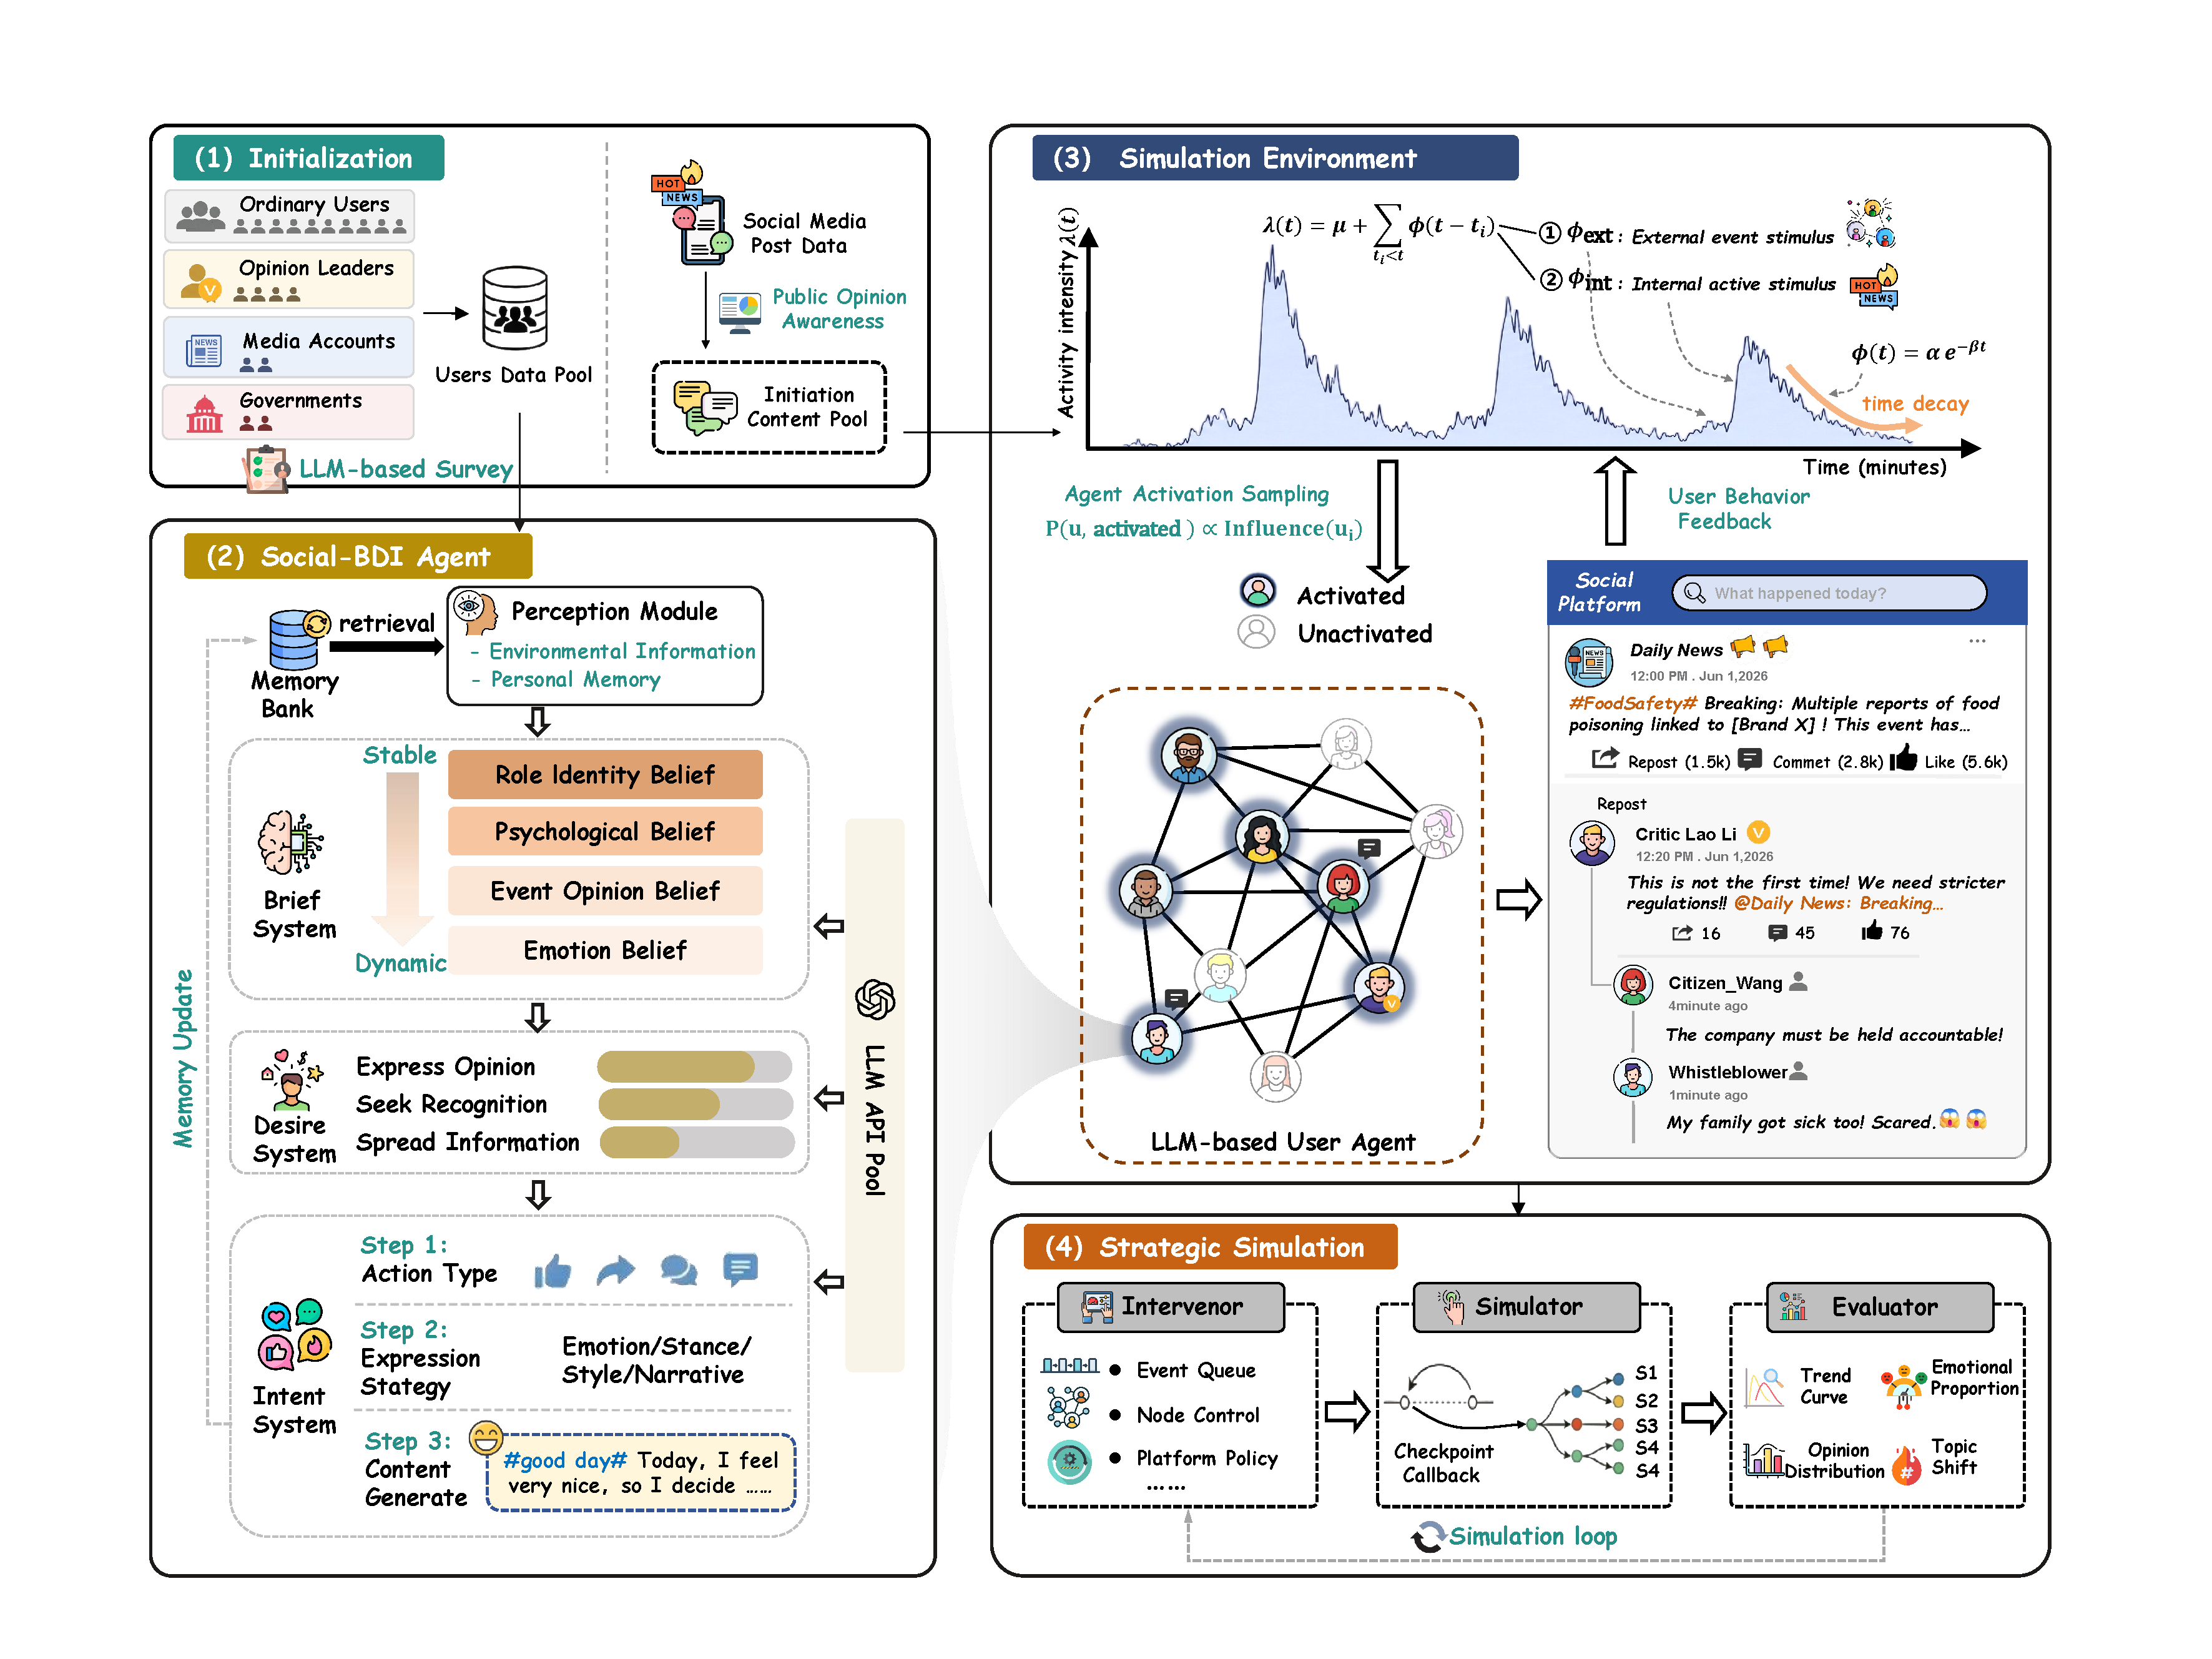
\includegraphics[width=0.85\textwidth]{framework_overview.pdf}
\caption{POSIM框架总体架构。(1)~初始化模块基于真实用户数据和博文数据对智能体和环境的初始化；(2)~Social-BDI智能体架构实现感知$\to$信念$\to$欲望$\to$意图$\to$行为的认知决策链路；(3)~仿真环境由霍克斯自激点过程驱动的时间引擎控制智能体激活，虚拟社交媒体平台提供个性化推荐和社交网络交互；(4)~策略推演由干预器、模拟器以及评估器共同构成。}
\label{fig:framework}
\end{figure*}

\subsection{POSIM框架概览}\label{subsec:overview}

POSIM的整体架构如图~\ref{fig:framework}所示，由\textbf{Social-BDI智能体架构}、\textbf{仿真环境}和\textbf{策略推演}三个核心组件构成，三者分别对应“谁在参与”“在何种环境中参与”以及“如何利用仿真支撑决策”三个关键问题。

在智能体层面（第\ref{subsec:agent}节），POSIM为每个仿真用户构建了受BDI认知理论启发的Social-BDI架构，该架构将认知过程显式分解为信念更新、欲望生成和意图规划三个独立子系统，各子系统以LLM为推理引擎依次运行，形成从环境感知到行为输出的完整且可追溯的认知决策链路。信念子系统维护角色身份、心理认知、事件观点和情绪激发四个层次的认知状态，为下游决策提供个性化的认知锚定；欲望子系统将信念状态映射为带有强度权重的行为动机；意图子系统通过三级思维链将动机转化为具体的行为类型、表达策略和文本内容。基于该架构，我们进一步定义了普通社交用户、意见领袖、媒体和政府四类异质性智能体，它们共享同一套认知管线，但通过差异化的角色引导提示词自然产生符合各自社会角色特征的行为表现。

在环境层面（第\ref{subsec:env}节），POSIM构建了包含社交网络与信息曝光机制的虚拟社交媒体环境，为智能体提供贴近真实平台的信息环境。在此基础上，框架引入基于霍克斯自激点过程的时间动力学引擎，将外生事件冲击与内生用户交互统一建模为动态变化的群体活跃强度，使智能体与环境在分钟级时间分辨率下持续耦合，自然再现舆情的“爆发—持续—衰退”多阶段演化模式。

在策略推演层面（第\ref{subsec:strategy}节），干预器、仿真器和评估器三个功能模块协同工作，支持从事件注入、节点控制到平台策略调整的多粒度干预，并通过检查点回调机制实现反事实推理，为舆情治理的策略评估提供定量支撑。

以下各节将依次详细介绍上述三个核心组件的设计与实现。



\subsection{Social-BDI智能体架构}\label{subsec:agent}

传统的反应式智能体遵循简单的感知到行动模式，仅作为无状态的行为生成器，无法捕捉社交用户决策中涉及的复杂认知机制。考虑到社交媒体用户的行为决策受情绪驱动、认知偏差和社交影响等多重非理性因素的交互作用，且情绪与意图的深度耦合是危机事件演化的核心动力~\citep{myint2024crisis_mtl_intent}，我们在经典BDI（信念-欲望-意图）认知架构~\citep{bratman_intention_1987,rao_bdi_1995}的基础上，融入情感维度，提出Social-BDI智能体架构，将情绪唤醒与认知偏差等非理性因素融入分层认知框架。Social-BDI的核心特征体现在两方面。其一，智能体具有显式的自我认知状态，每一步决策均基于可观测的认知状态变化；其二，智能体的认知过程本身是可审查的多阶段决策链~\citep{wei_chain_2022}，而非单次黑箱调用。认知链路形式化为：
\begin{equation}
\underset{\text{Perception}}{P_t} \longrightarrow \underset{\text{Belief}}{B_t} \longrightarrow \underset{\text{Desire}}{D_t} \longrightarrow \underset{\text{Intention}}{I_t} \longrightarrow \underset{\text{Action}}{A_t}
\end{equation}

该架构以LLM为认知推理引擎，包含信念子系统、欲望子系统和意图子系统三个核心模块。三个子系统在每个决策周期内依次运行，各自接收上游输出作为输入，形成从环境感知到行为输出的完整且可追溯的认知链路。

\subsubsection{信念子系统}

信念是智能体对外部世界和自身状态的动态认知表征，构成一切决策推理的基础。社会心理学研究表明，个体的不同认知层次具有不同的稳定性，核心人格特质在短期内高度稳定，而对特定事件的观点和即时情绪则随信息输入快速变化。基于这一认知分层特性，并结合真实社交媒体用户的实际特点，我们设计了层次化的信念体系$B = \langle B^{id}, B^{psy}, B^{evt}, B^{emo} \rangle$，四类信念按认知修正难度从高到低排列。

\textbf{角色身份信念}$B^{id}$表征智能体的固有基础认知，包括人口学属性（性别、地域）、社交属性（粉丝规模、认证类型）和身份属性（职业、兴趣标签）等，在仿真周期内保持恒定。初始化时，从真实社交媒体平台采集用户的基础信息及历史发布内容，利用LLM进行结构化推断，以第一人称自述的自然语言形式生成角色身份描述。该信念在仿真过程中不会更新，作为智能体人格一致性的锚定层。

\textbf{心理认知信念}$B^{psy}$表征智能体在舆情参与中的深层心理特征与认知倾向。社会心理学研究表明，社交用户在面对网络事件时表现出从众、成见、冲动、偏执等典型心理现象~\citep{buckels2014trolls}。基于对多起真实舆情事件中用户行为模式的分析，我们将用户心理特征归纳为自我实现型、猎奇探究型、减压宣泄型、仇官仇富型、跟风从众型等典型模式。每种模式下均配有从大量真实舆情数据中总结的预定义心理认知条目，例如仇官仇富型包含“主流媒体未报道的往往才是真相”“富人的财富来源存疑”等认知描述，减压宣泄型则包含“看热闹不嫌事大”“骂得越狠越解气”等条目。心理认知信念以结构化文本列表形式存储，初始化时基于采集的真实用户历史行为内容，通过LLM从预定义心理特征池中进行个性化采样与适配，为每个智能体匹配与其历史表现最为吻合的心理认知组合。心理认知信念在仿真过程中保持高度稳定，反映了深层心理特质的抗变性。

\textbf{事件观点信念}$B^{evt}$表征智能体对特定舆情事件中各参与主体的事实认知、背景理解和观点立场。与前两类信念不同，事件观点信念随舆情发展动态演化，新信息的摄入、他人观点的影响和事件进展均可能导致观点的修正或强化。每条事件观点采用结构化四元组表示$\langle t, \text{subject}, \text{opinion}, \text{reason} \rangle$。初始化时，基于用户在事件爆发前的历史发布内容，通过LLM驱动的结构化深度访谈机制提取用户对各参与主体的初始观点倾向，例如针对事件中的涉事主体，访谈会提出“对于涉事方X，你当前对其持怎样的看法？”等引导性问题，由LLM结合用户历史行为推断其初始立场与理由。

\textbf{情绪激发信念}$B^{emo}$基于认知行为理论中的ABC模型~\citep{ellis_reason_1962}，强调认知评价对情绪反应和后续行为的中介作用。我们采用Ekman的六维基本情感分类框架~\citep{ekman_basic_1992}，将情绪状态表征为连续向量$\mathbf{e} = [e_{\text{hap}}, e_{\text{sad}}, e_{\text{ang}}, e_{\text{fear}}, e_{\text{sur}}, e_{\text{dis}}]^\top \in [0,1]^6$，分别对应快乐、悲伤、愤怒、恐惧、惊讶和厌恶六种基本情绪。情绪状态的更新受三个机制驱动。\textbf{时间衰减}参照心理学中情绪的自然消退规律，情绪强度随时间按指数衰减
\begin{equation}
\mathbf{e}_i(t) = \mathbf{e}_i(t_0) \cdot e^{-\lambda_e(t-t_0)}
\end{equation}
\textbf{内容刺激}指智能体浏览的推荐内容中蕴含的情感色彩对其情绪产生增量影响$\mathbf{e}_i \leftarrow \mathbf{e}_i + \eta \cdot \mathbf{s}_{content}$，其中$\eta$为刺激系数。\textbf{社交传染}基于在线社交网络中的情绪传染理论~\citep{hatfield_emotional_1994,kramer_experimental_2014,fan2023emotional_contagion}，智能体的情绪受其社交邻居的情绪状态影响
\begin{equation}
\mathbf{e}_i \leftarrow (1-\rho) \cdot \mathbf{e}_i + \rho \cdot \bar{\mathbf{e}}_{\text{neighbor}}
\end{equation}
其中$\rho$为传染强度系数，$\bar{\mathbf{e}}_{\text{neighbor}}$为邻居情绪的加权平均。

\textbf{信念更新机制。}每时间步，我们会利用LLM对智能体的信念子系统进行更新。信念更新基于外部环境感知$P_t$与历史行为记忆$M_t$双通道信息输入，输出为更新后的心理认知、事件观点和情绪激发信念。历史记忆采用流式记忆库存储，检索时使用同时兼顾时间衰减与语义相似度的加权打分函数：
\begin{equation}
R(m, t) = \alpha_{\mathrm{rec}} e^{-\gamma(t - t_m)} + (1-\alpha_{\mathrm{rec}})\,\text{sim}(q, m),
\label{eq:mmr}
\end{equation}
其中$\text{sim}(\cdot,\cdot)$为基于预训练编码器的余弦相似度，$\alpha_{\mathrm{rec}}\in[0,1]$控制近因性与相关性之间的权衡。然而，真实社交用户的信念更新并非完全理性的信息整合过程，而是系统性地受到多种认知偏差的影响。例如，用户往往倾向于选择性接受与既有观点一致的信息而忽略矛盾证据（\textit{确认偏差}），在形成观点时过度依赖最先接触到的信息（\textit{锚定效应}），在高唤醒情绪状态下跳过理性分析而直接基于情绪做出判断（\textit{情绪优先推理}），以及将复杂的社会事件归结为单一原因或个体责任（\textit{简单归因倾向}）。这些认知偏差在舆情场景中尤为显著，是驱动非理性话语和群体极化的重要心理机制。为此，我们在LLM推理过程中通过提示词显式引入上述认知偏差引导，使智能体的信念更新过程更贴近真实用户的认知特征。信念更新的整体形式为：
\begin{equation}
B_{t+1} = f_{\text{LLM}}(B_t, P_t, M_t, \Phi)
\label{eq:belief_update}
\end{equation}
其中$\Phi$为嵌入提示词中的认知偏差引导。更新主要作用于$B^{evt}$和$B^{emo}$两个快速变化层，同时以较小变化缓慢调整$B^{psy}$；$B^{id}$作为身份锚点在仿真过程中保持不变。

\begin{table}[!t]
\centering
\caption{Hierarchical belief system design. Beliefs are ordered by decreasing cognitive resistance to change: identity beliefs remain fixed, while emotional beliefs update at every step.}
\label{tab:belief}
\scriptsize
\renewcommand{\arraystretch}{1.15}
\begin{tabular}{@{}p{1.15cm}p{1.85cm}p{1.05cm}p{2.3cm}@{}}
\toprule
\textbf{Belief} & \textbf{Representation} & \textbf{Stability} & \textbf{Generation Method} \\
\midrule
$B^{id}$ \newline Identity & First-person natural language narrative & Fixed & LLM init.\ from real user profiles \\
\addlinespace
$B^{psy}$ \newline Psychology & Structured text entry list & Highly stable & LLM + psychological trait pool \\
\addlinespace
$B^{evt}$ \newline Event view & Structured tuple $\langle t, \text{subj}, \text{op}, \text{rsn}\rangle$ & Dynamic & LLM inference at each decision step \\
\addlinespace
$B^{emo}$ \newline Emotion & Six-dim.\ vector $\mathbf{e}\!\in\![0,1]^6$ & Rapid & LLM appraisal + decay \& contagion \\
\bottomrule
\end{tabular}
\end{table}

\subsubsection{欲望子系统}

欲望子系统承担从认知状态到行为动机的桥梁角色，是Social-BDI架构中连接“智能体如何理解世界”与“智能体想要做什么”的关键环节。在经典BDI理论中，欲望（Desire）被定义为智能体希望达成的目标状态~\citep{bratman_intention_1987}；在社交媒体语境下，我们将其操作化为驱动用户参与舆情讨论的内在动机。社交媒体用户的参与动机高度多样化且因人而异，同一条新闻可能激发一个用户的正义感而激发另一个用户的猎奇心理，这种动机的异质性难以用固定规则覆盖，因此我们利用LLM的常识推断能力，基于智能体当前的信念状态自动推断行为驱动力。

每个时间步，欲望子系统接收更新后的信念状态$B_{t+1}$和当前感知$P_t$作为输入，输出一组带有强度权重的动机描述：
\begin{equation}
D_t = \{(d_1, w_1), (d_2, w_2), \ldots, (d_n, w_n)\}, \quad w_i \in [0, 1]
\end{equation}
其中$d_i$为自然语言描述的动机类型，$w_i$为对应的强度权重，反映该动机在当前认知状态下的驱动力大小。传播学中的使用与满足理论~\citep{katz_uses_1973}指出，受众并非被动的信息接收者，而是基于自身需求主动选择和使用媒介内容以获得心理满足。受这一理论启发，我们认为社交媒体用户参与舆情讨论同样受多元内在需求驱动，并据此考虑和归纳了智能体可能产生的多种类型欲望目标。普通社交用户常见的动机包括情绪宣泄（将不满和焦虑通过发言释放）、正义倡导（为弱势方发声或推动问题解决）、从众跟风（跟随热门话题参与讨论以融入群体）和猎奇探究（关注事件新进展以满足好奇心）；意见领袖则更多表现出自我表达（展示独立见解以巩固影响力）和议程设置（引导公众关注特定议题）等动机。动机的具体组合和强度分布并非预设，而是由LLM根据信念状态动态推断，例如，当智能体的情绪激发信念$B^{emo}$中愤怒维度较高且事件观点信念$B^{evt}$中持强烈负面立场时，情绪宣泄和正义倡导动机往往获得较高权重；而当心理认知信念$B^{psy}$以猎奇探究为主导时，信息获取动机则更为突出。

动机列表为下游意图子系统的行为规划提供显式的目标约束，高权重动机引导智能体选择与之匹配的行为类型和表达策略，例如当情绪宣泄动机强度最高时，智能体更倾向于选择短评论和激烈的情感表达；当自我表达动机占主导时，则倾向于发布长原创博文并采用理性分析的表达风格。欲望生成函数形式化为：
\begin{equation}
D_t = g_{\text{LLM}}(B_{t+1}, P_t)
\end{equation}

这一设计的核心价值在于引入了显式的动机中间层，使信念状态不再直接映射为行为输出，而是先经由欲望子系统生成结构化的动机表征，再由意图子系统据此规划具体行为。消融实验（第\ref{sec:exp}节）将表明，移除欲望模块后内容层指标退化最为严重，验证了动机层对于驱动非理性话语表达的不可替代性。

\subsubsection{意图子系统}

意图子系统作为认知链路的最终决策环节，承担层级行为规划器的角色。根据社交媒体平台的交互规则，我们将行为类别约束为点赞、直接转发、转发带评论、短评论、长评论、短原创博文和长原创博文等原子操作。与传统的单步行为生成不同，意图子系统采用多级思维链机制，将行为决策分解为三个递进的推理层级。

\textbf{第一级——行为类别与目标对象选择。}LLM根据信念状态和欲望强度分布，从几种原子操作中选择行为类别，并确定互动的目标对象。该层级决定做什么和对谁做。

\textbf{第二级——表达策略规划。}对于需要生成文本内容的行为，系统在四个通用维度上规划表达策略：\textit{情绪维度}确定主导情绪类型与强度等级；\textit{立场维度}确定对目标主体的支持、反对或中立立场及其强度；\textit{风格维度}选择理性分析、讽刺调侃、情绪攻击、共情理解、质疑求证等表达风格；\textit{叙事维度}选择事实罗列、标签化、行动呼吁、权威引用等叙事策略。每个维度均包含多种候选选项，由LLM根据当前认知状态自主选择最合适的组合。该层级决定以什么方式表达。

\textbf{第三级——内容生成。}基于前两级决策的约束，生成符合角色特征的具体文本内容，包括正文、话题标签和提及。该层级决定具体说什么。

这种三级分解设计为内容生成提供了显式的策略约束，避免了LLM在无引导下倾向于生成平均化的温和文本；同时每一级的决策结果均被记录，使得行为的生成过程完全可追溯。整体意图生成过程形式化为：
\begin{equation}
I_t = h_{\text{LLM}}(B_{t+1}, D_t, P_t)
\end{equation}
其中$I_t = \{(a_j, o_j, s_j, c_j)\}_{j=1}^{m}$为行为序列，每个元素包含行为类型$a_j$、目标对象$o_j$、表达策略向量$s_j = (\text{emotion}, \text{stance}, \text{style}, \text{narrative})$和生成内容$c_j$。

\subsubsection{异质性智能体}

真实舆情演化涉及普通社交用户、意见领袖、媒体和政府等多类主体的复杂交互~\citep{chen_evolution_2025,wu_public_2023}。本节介绍的四种异质性智能体类型，均基于上述Social-BDI认知架构进行统一构建，即所有类型的智能体共享同一套从感知到信念、欲望、意图再到行为的完整认知管线，使用相同的信念更新、欲望生成和意图规划模块。不同智能体类型之间的行为差异，并非通过修改认知架构本身或引入额外的决策规则实现，而是仅通过各自专属的角色引导提示词注入不同的社会角色特征（如身份定位、发言风格、关注重点等），使同一认知架构在不同角色约束下自然产生差异化的行为表现。这一设计确保了行为异质性的来源是角色信念的差异而非架构的差异，从而保持了框架的统一性和可解释性。

\textbf{普通社交用户}是舆情参与的绝对主体，其社交行为主要受个人信念与即时情绪的交互影响。普通用户的语言风格通常较为口语化和碎片化，在高唤醒情绪驱动下容易产生冲动性表达。

\textbf{意见领袖}在二级传播理论~\citep{katz_personal_1955}中被视为信息流动的关键中介，拥有较大的粉丝基础和社会影响力。其观点输出往往具有较强的独立性和议程设置效应，对下游普通用户的信念更新和行为决策具有显著的引导作用。

\textbf{媒体智能体}承担信息采集与传播的社会功能，注重内容的时效性、准确性和权威性。其语言表达相对规范和克制，主要通过发布新闻报道、事件进展和深度评论等形式参与舆情传播，在事件关键节点上起到信息确认和议程框定的作用。

\textbf{政府智能体}代表官方立场与公共治理视角，承担政策解读、舆论引导和信息公开等社会职能。其发言频率较低但权威性较高，通常在事件发酵到一定程度后发布官方声明或回应，对舆情走势具有较强的转折性影响。

四种智能体的具体行为模式并非预先设定，而是在各自的角色引导提示词约束下由Social-BDI认知链路自主生成。

完整的认知链路实例详见附录~\ref{app:prompts}中的提示词模板。

\subsection{仿真环境}\label{subsec:env}

仿真环境是智能体感知和交互的虚拟社交媒体平台，其设计目标是在保持计算可行性的前提下真实再现社交平台的信息流动机制和时间动力学特性。如图~\ref{fig:framework}所示，仿真环境由时间引擎和社交网络与信息流机制两大组件构成，前者负责时序调度，后者负责信息分发，二者协同为智能体提供完整的虚拟社交媒体体验。

\subsubsection{时间引擎}

真实舆情事件中的用户活跃度呈现高度不均匀的时间分布，一条爆炸性新闻可在数分钟内引发数千条转发，而事件间歇期的活跃度则大幅回落。传统仿真系统普遍采用固定时间步长的均匀激活模式，每步激活固定数量的智能体，这种设计无法再现真实舆情中事件驱动的活跃度突变特征。

为此，POSIM引入了基于霍克斯自激点过程的\textbf{时间引擎}作为仿真环境的时序调度基础。该引擎的核心思想在于，群体活跃强度并非预设的固定值，而是由外生事件冲击和内生用户交互共同驱动的动态过程。具体而言，我们采用霍克斯自激点过程~\citep{hawkes_spectra_1971}对群体活跃强度进行建模。霍克斯过程的直觉可以类比为一场“传染”，也就是每一次事件发生后都会短暂地提高后续事件发生的概率，就像一条热门微博引发的讨论会在短时间内刺激更多用户参与，随后这种刺激效应逐渐衰减。形式化地，其条件强度函数定义为：
\begin{equation}
\lambda(t) = \mu + \sum_{t_i < t} \phi(t - t_i)
\label{eq:hawkes}
\end{equation}
其中$\mu$为基础活跃率，反映舆情低谷期的背景发博行为；$\phi(t) = \alpha e^{-\beta t}$为指数衰减的激励核函数，刻画每次历史事件对当前活跃度的短期抬升效应，即事件刚发生时激励最强，随后随时间指数衰减，所有历史事件的激励叠加构成当前时刻的总活跃强度。

本文我们的关键设计在于将激励项分为\textbf{外生事件激励}$\phi_{ext}$和\textbf{内生活跃激励}$\phi_{int}$两类来源（见图~\ref{fig:framework}）。外生事件激励对应外部新闻发布、官方声明等关键事件刺激，具有较大的激励强度和较慢的衰减速率，能够在短时间内大幅抬升群体活跃水平并维持较长的影响窗口；内生活跃激励对应用户间的互动行为（转发、评论、点赞），具有较弱的激励强度和较快的衰减速率，体现了社交传播中滚雪球式的自激效应。两类激励的叠加使得仿真系统能够自然产生与真实舆情一致的“爆发—持续—衰退”活跃模式。

在此基础上，我们进一步结合大量舆情事件发生规律，引入昼夜节律调制机制，通过一个以24小时为周期的调制函数对霍克斯强度进行缩放。在每个仿真步$\Delta t$内，系统根据调制后的强度函数通过泊松采样确定本步激活的智能体数量$N_t \sim \text{Poisson}(\lambda_{adj}(t)\, N_{\text{scale}})$，被激活的智能体通过基于历史活跃度的加权采样确定。整个时间引擎的参数配置详见附录~\ref{tab:hawkes_params}。

\subsubsection{社交网络与信息流机制}

在时间引擎确定每步激活的智能体后，社交网络与信息流机制共同决定了智能体看到什么和被什么博文吸引，直接影响其后续的交互行为。

\textbf{社交网络。}社交网络是信息流动的底层基础设施，POSIM维护粉丝关注网络、实时转发网络和实时评论网络三层有向关系结构。粉丝关注网络记录用户间的单向关注关系，构成推荐系统中关系链内容的来源范围；转发网络和评论网络在仿真过程中随智能体交互动态生长，每当智能体执行转发或评论行为时，系统自动记录交互双方的关系并更新网络拓扑。

\textbf{内容推荐。}基于社交网络关系，内容推荐系统维护一个全局内容池，所有智能体发布的博文、评论和转发均实时写入该池，并由预训练语义编码器（BGE-small-zh\footnote{\url{https://huggingface.co/BAAI/bge-small-zh-v1.5}}）生成向量表征。为抑制LLM生成内容的同质化倾向，系统对新入池内容执行基于余弦相似度的语义去重。候选内容的来源分为两个通道。\textbf{关系链通道}从用户关注列表对应的博文中召回，保证社交关系的信息传递作用；\textbf{公域通道}从全局内容池中召回，模拟平台算法对跨圈层内容的分发能力。两个通道的候选内容合并后，系统按以下三个维度加权计算推荐得分。\textbf{同质性}$H(u,p)$衡量用户历史兴趣向量与候选内容语义向量的余弦相似度，反映信息茧房效应~\citep{cinelli_echo_2021}；\textbf{热度}$P(p)$基于点赞、转发和评论三类互动信号的归一化加权得分，体现平台对高互动内容的流量倾斜；\textbf{新鲜度}$R(p)$通过指数时间衰减函数计算，确保近期内容获得更高的曝光概率。最终推荐得分为：
\begin{equation}
S_{exp}(u, p) = \alpha \cdot H(u, p) + \beta \cdot P(p) + \gamma \cdot R(p)
\label{eq:recommend}
\end{equation}
其中$\alpha$、$\beta$、$\gamma$为可调权重参数（具体取值见附录表~\ref{tab:rec_params}）。排序完成后，系统在推荐列表中保留一定比例的探索位用于随机推荐，以打破过度的信息茧房效应~\citep{bail_opposing_2018}。推荐历史记录机制确保同一内容不会在短期内重复推送给同一用户。

\textbf{热搜榜单。}系统自动统计仿真中涌现的话题标签热度，综合互动信号与时间衰减定期更新排名，排名靠前的话题注入智能体的感知输入，模拟真实平台中热搜对注意力聚焦的放大效应。

\subsection{策略推演}\label{subsec:strategy}

POSIM不仅是一个仿真器，更是一个支持策略评估的计算实验平台。在舆情治理实践中，决策者通常需要回答“如果采取某种干预措施，舆情走势将如何变化”这类反事实问题。如图~\ref{fig:framework}右下所示，POSIM的策略推演框架由\textbf{干预器}（Intervenor）、\textbf{仿真器}（Simulator）和\textbf{评估器}（Evaluator）三个功能模块协同完成。

\textbf{干预器}是连接外部治理意图与仿真内部状态的统一接口层，提供三个粒度的注入方式：\textbf{事件队列}（Event Queue）在指定时间点向全体智能体广播外部事件，例如注入一条官方声明或突发新闻；\textbf{节点控制}（Node Control）针对特定智能体进行定点干预，例如调整某一意见领袖的信念状态以模拟引导策略；\textbf{平台策略}（Platform Policy）修改仿真环境的运行参数，例如调整推荐算法权重或限制特定内容的传播范围。三类接口可单独使用或组合叠加，为研究者提供从微观个体到宏观环境的全方位干预能力。

\textbf{仿真器}负责将干预方案转化为可执行的计算实验。其核心机制是\textbf{检查点回调}（Checkpoint Callback），系统在仿真运行过程中周期性保存完整的状态快照，研究者可从任意检查点加载历史状态并注入不同的干预方案，从而在完全相同的初始条件下生成多条平行演化轨迹。这一设计天然支持反事实推理，只需从同一检查点分叉，分别施加不同干预或不施加干预，即可直接对比各策略的效果差异。

\textbf{评估器}与仿真引擎完全解耦，通过标准化数据接口读取仿真日志，从热度曲线、情感比例、观点分布、话题迁移等指标出发，对仿真输出进行多维量化评估，全面刻画舆情演化状态。评估结果可直接反馈用于指导下一轮干预方案的调整与优化。

\textbf{LLM资源调度。}大规模仿真涉及大量LLM调用，框架通过统一的API资源池管理多个LLM端点，支持多模型混合驱动。在用途路由方面，资源池为信念更新、欲望生成、行为决策等不同用途维护独立的模型选择计数器，支持按用途指定不同的LLM端点，兼顾推理质量与成本效率。此外，为避免LLM在大规模调用中产生同质化输出，系统对每次调用的采样参数进行随机扰动以增强输出多样性，具体包括Temperature扰动$T' = T + \epsilon_T$（$\epsilon_T \sim \mathcal{U}(-0.1, 0.1)$）、Top-p扰动$p' = p + \epsilon_p$（$\epsilon_p \sim \mathcal{U}(-0.05, 0.05)$），并随机注入频率惩罚和存在惩罚参数以增加词汇和话题多样性。资源池同时实现了端点级并发控制、轮询式负载均衡、故障自动检测与转移以及调用频率限制。

\textbf{模块化架构。}舆情仿真研究的一个核心挑战在于不同研究场景对认知模型、时间动力学和评估维度的需求各异，单一的固化架构难以适应多元化的研究目标。为此，POSIM在设计之初即遵循\textbf{关注点分离}原则，将智能体认知、仿真环境和策略推演三大核心关注点封装为相互独立的功能模块，模块间仅通过语义明确的结构化状态进行信息传递，而非共享内部实现细节。这一设计理念使得每个模块的演化不受其他模块约束，例如研究者可以在保持仿真环境和评估体系不变的前提下，将Social-BDI认知架构替换为其他决策模型以探索不同的认知假说，或在保持智能体架构不变的条件下切换时间引擎以适配不同的时间尺度需求，亦可接入新的评估维度以支撑特定的研究问题。这种面向研究可扩展性的架构设计，使POSIM能够从单一的舆情仿真工具演进为一个支撑多种社会仿真研究范式的通用计算实验平台。

% ============================================================
% 第4节 三层递进验证框架
% ============================================================
\section{验证框架}\label{sec:validation}

本文的验证框架受系统工程领域经典的V\&V（Verification and Validation）原则启发~\citep{sargent_verification_2013}，我们将模型评估分为验证和确认两个互补维度，验证回答（“我们是否正确地构建了模型？”）的问题，而确认则回答（“模型结果是否准确？”）的问题。基于这一原则，验证遵循三层递进的过程，其中微观行为机制校准和宏观现象涌现校准属于验证层面，统计结果一致性校准属于确认层面。

\textbf{微观行为机制校准}（第\ref{subsec:micro}节）验证智能体是否按照设计意图做出认知上可解释的决策。该层次关注的是仿真系统的内部机制正确性，从三个递进维度进行考察。\textit{认知行为链一致性}检验智能体从信念更新到行为输出的认知链路是否完整、连贯且符合逻辑，即每一步决策是否能追溯到明确的认知依据；\textit{人格稳定性}评估智能体在多轮交互中是否保持与其角色身份一致的行为风格，而非随机漂移；\textit{决策抗扰性}测试在输入信息发生语义等价扰动时，智能体的决策是否保持稳定，以验证认知锚定机制的有效性。微观机制的正确性是整个验证体系的基石，因为只有微观机制正确，宏观涌现才具有因果上的可解释性。

\textbf{宏观现象涌现校准}（第\ref{subsec:macro}节）验证微观机制能否涌现出符合社会科学理论预期的宏观现象。该层次将仿真视为一个计算实验，从四个维度检验系统是否能在无显式宏观编程的前提下自发产生社会科学理论所预测的群体行为模式，包括舆情生命周期的多阶段演化特征、多类型智能体的系统性行为异质性、情绪唤醒自增强与极化效应、以及网络拓扑的无标度特征与信息级联的幂律分布。涌现现象的出现为微观机制的合理性提供了间接而有力的佐证。

\textbf{统计结果一致性校准}（第\ref{subsec:stat}节）在机制校准后，验证仿真输出是否在统计意义上准确再现真实舆情动态。该层次通过与真实舆情数据在行为层（行为类型分布与活跃度曲线）、内容层（话语非理性分布、词汇多样性与情感倾向）和拓扑层（网络结构与信息级联模式）三个维度共九个定量指标进行系统性比对，从而建立仿真的统计可信度。

% ============================================================
% 第5节 实验
% ============================================================
\section{实验}\label{sec:exp}

\subsection{数据集}

我们从新浪微博平台采集了三个覆盖原创博文、转发与评论全链路交互的真实舆情事件数据集，三个事件分别属于社会争议、校园事件和食品安全类别，涵盖了从短时爆发到长周期多阶段演化的不同舆情模式。\textbf{天价耳环事件}（LE）发生于2025年5月，某演员发布成人礼照片中佩戴的绿色耳饰被网友指认为疑似价值230万元的奢侈品牌耳环，迅速引发公众对明星炫富行为与青少年价值观导向的激烈争议，话题多次登上微博热搜，舆情呈现典型的短时集中爆发模式。\textbf{武汉大学图书馆事件}（WL）起源于2023年7月武汉大学图书馆自习区的一起性骚扰指控纠纷，2025年7月法院一审判决再次引爆舆论，围绕司法公正、校园安全与性别议题展开大规模讨论，舆情经历了从沉寂到复燃的长周期多阶段演化。\textbf{西贝预制菜事件}（XF）于2025年9月因网红企业家公开指控西贝餐饮大量使用预制菜而引发，双方持续交锋带动公众对食品安全和消费者知情权的广泛关注，舆情呈现多方博弈驱动的持续发酵模式。

本文选取各事件舆情爆发与演化最为集中的核心时段进行精准模拟，以在有限计算资源下最大化仿真的信息密度。数据经过去重、低活跃用户过滤和无关内容清洗后的描述性统计见表~\ref{tab:dataset}。仿真时间精度为10分钟/步。智能体的信念初始化基于每个用户在仿真起始时间之前的历史发布内容，依次构建角色身份信念、心理认知信念、事件观点信念和初始情绪向量，形成完整的个性化Social-BDI信念系统。

\begin{table}[!t]
\centering
\caption{Descriptive statistics of three public opinion event datasets.}
\label{tab:dataset}
\footnotesize
\renewcommand{\arraystretch}{1.05}
\begin{tabular}{@{}lccccc@{}}
\toprule
\textbf{Event} & \textbf{\#Users} & \textbf{\#Posts} & \textbf{Duration} & \textbf{\#Steps} & \textbf{Category} \\
\midrule
LE & 1,530 & 34,218 & ${\sim}$46h & 276 & Social Controversy \\
WL & 1,843 & 51,647 & ${\sim}$190h & 1,140 & Campus Incident \\
XF & 1,987 & 14,892 & ${\sim}$71h & 426 & Food Safety \\
\bottomrule
\end{tabular}
\par\vspace{2pt}
{\scriptsize\fontspec{Times New Roman}\selectfont
\textit{Note}: LE = Luxury Earring; WL = WHU Library; XF = Xibei Prepared Food.}
\end{table}

\subsection{微观行为机制验证}\label{subsec:micro}


\subsubsection{对比方法}

微观验证聚焦于单个智能体的认知决策质量，因此对比方法均在相同的输入条件下，考察不同认知架构对决策可解释性、人格一致性和鲁棒性的影响。设置四种决策方法：\textbf{Direct-Nothink}使用非思考版模型Qwen2.5-7B-Instruct\footnote{\url{https://huggingface.co/Qwen/Qwen2.5-7B-Instruct}}，将环境信息和角色描述拼接为单次提示，直接要求模型输出行为决策，不进行任何显式的认知推理过程。\textbf{Direct-Think}将模型升级为较强的Qwen3-8B\footnote{\url{https://huggingface.co/Qwen/Qwen3-8B}}思考版模型，同样采用单次提示直接输出。\textbf{CoT}使用与Social-BDI相同的基座模型Qwen2.5-7B-Instruct，在单次LLM调用内通过思维链提示串联完成信念推断、欲望分析和行为决策的全过程，信念-欲望-意图三个阶段在同一上下文窗口中顺序完成而非独立模块化。\textbf{Social-BDI}为本文提出的方法，同样使用Qwen2.5-7B-Instruct作为基座模型，将认知过程分解为信念更新、欲望生成和意图规划三个独立模块，每个模块由单独的LLM调用完成，模块间通过结构化中间状态传递信息。

\subsubsection{评估设置与结果}

随机抽取$N=100$名用户作为智能体，仿真共进行$T=12$轮，四种方法在相同条件下运行。三个评估维度包括：\textbf{认知行为链一致性}从认知链完整性、情绪动态合理性、动机-行为对齐度和信息整合能力四个子维度进行0--5分等级评分；\textbf{人格稳定性}评估LLM基于行为轨迹反推智能体身份描述的相似度（0--1）；\textbf{决策抗扰性}对输入进行语义等价扰动后评估决策稳定性（0--1）。三种评估均由稳定超参数下的大模型提示给出输出，最终结果见表~\ref{tab:micro}。

\begin{table}[!t]
\centering
\caption{Micro-level behavioral mechanism validation results (mean$\pm$std).}
\label{tab:micro}
\renewcommand{\arraystretch}{1.05}
\resizebox{\columnwidth}{!}{%
\scriptsize
\begin{tabular}{@{}lccc@{}}
\toprule
\textbf{Method} & \makecell{\textbf{Cognitive-Behavior}\\\textbf{Chain Consistency} (0--5)\,$\uparrow$} & \makecell{\textbf{Personality}\\\textbf{Stability} (0--1)\,$\uparrow$} & \makecell{\textbf{Decision}\\\textbf{Robustness} (0--1)\,$\uparrow$} \\
\midrule
Direct-Nothink & 1.47$\pm$0.50 & 0.478$\pm$0.263 & 0.629$\pm$0.240 \\
Direct-Think & 1.75$\pm$0.43 & 0.448$\pm$0.269 & 0.603$\pm$0.299 \\
CoT & 3.09$\pm$0.29 & 0.516$\pm$0.272 & 0.541$\pm$0.356 \\
\rowcolor{grayrow}
\textbf{Social-BDI (Ours)} & \textbf{4.64}$\pm$\textbf{0.48} & \textbf{0.661}$\pm$\textbf{0.215} & \textbf{0.695}$\pm$\textbf{0.213} \\
\bottomrule
\end{tabular}%
}
\end{table}

Social-BDI在三个维度上全面优于所有基线方法。认知行为链一致性得分4.64显著高于CoT的3.09（$p < 0.001$），表明分层认知架构产生的决策链路更加完整、连贯且符合逻辑。人格稳定性和决策抗扰性同样最优，验证了信念锚定机制的有效性。Direct-Think虽使用更强的思考版模型，但因缺乏认知结构约束，在人格稳定性和决策抗扰性上甚至不如Direct-Nothink，说明单纯的模型推理能力提升无法替代显式的认知架构设计。CoT虽在单次调用中串联了认知推理，但因缺少独立模块化的状态传递，其决策抗扰性反而最低（0.541），表明单次调用缺乏稳定的状态锚定，而Social-BDI通过显式信念状态提供了认知锚定效应。

\subsection{宏观现象涌现}\label{subsec:macro}

\subsubsection{舆情生命周期}

\begin{figure}[!t]
\centering
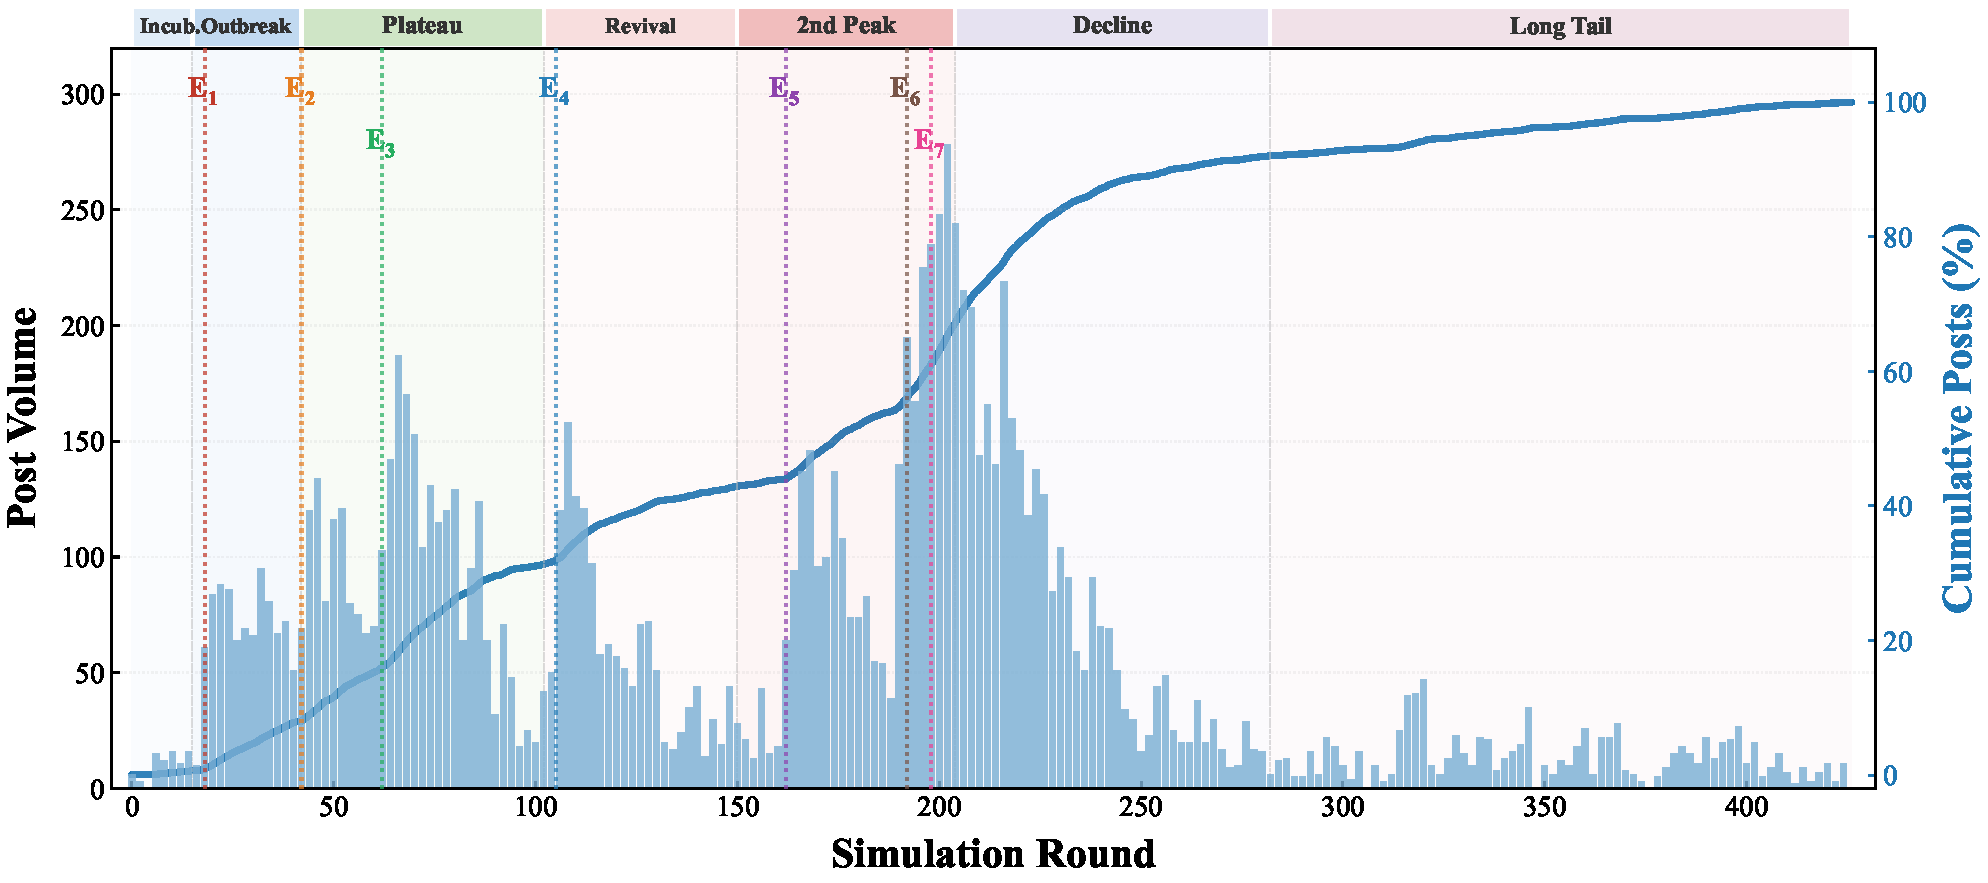
\includegraphics[width=\columnwidth]{fig_lifecycle_paper.pdf}
\caption{仿真舆情生命周期，展示发博量变化（柱状图，左轴）与累积发博百分比的S曲线（实线，右轴）。$E_1$--$E_7$标记外生事件注入时间点。}
\label{fig:lifecycle}
\end{figure}

舆情生命周期理论认为，网络舆情事件的发展并非匀速或单调的过程，而是呈现出具有阶段性特征的演化模式~\citep{guo_stochastic_2024,chen_evolution_2025}。典型的舆情生命周期包括爆发期（事件曝光引发公众集中关注，活跃度快速攀升）、平台期/持续期（热度趋于稳定或小幅波动）、可能的复燃期（新事件刺激引发二次爆发）以及衰退期（公众注意力转移，活跃度逐渐回落）。需要指出的是，并非所有舆情事件都严格遵循相同的阶段序列，短时爆发型事件可能直接从爆发进入衰退，而多方博弈型事件则可能经历多轮复燃。本节通过西贝预制菜事件（XF）的仿真结果，验证POSIM是否能够自发涌现出与该事件实际发展一致的生命周期模式。

如图~\ref{fig:lifecycle}所示，仿真清晰展现了该事件从爆发、平台、复燃到衰退的多阶段生命周期，且各阶段转换均可溯源至特定外生事件的因果驱动。$E_1$（西贝后厨漏勺视频曝光引发食品安全危机）注入后发博量迅速攀升，进入爆发期；$E_2$（罗永浩宣布暂时停战）后活跃度明显回落，进入平台期；$E_3$（餐饮业激辩预制菜定义）在平台期维持了一定的讨论热度，但未引发大规模爆发；$E_4$（创始人贾国龙群聊截图流出，称罗永浩为“网络黑社会”）重新点燃讨论，打破停战僵局；$E_5$（央媒集体发声点评）触发全程最大活跃度峰值，呈现典型的死灰复燃和官媒定调引发二次爆发的效应。累积发博百分比呈现S型增长曲线，与舆情传播学中S曲线扩散理论高度吻合~\citep{kong_exploring_2020}。

值得强调的是，上述多阶段生命周期模式并非预设规则驱动，而是由两层机制协同作用自发涌现的结果。在\textbf{环境层}，霍克斯点过程的自激机制使外生事件注入后群体活跃度呈现“激发—放大—衰减”的动态响应，外生事件提升基础激活强度，智能体发布的事件相关内容通过自激项$\sum \alpha e^{-\beta(t-t_i)}$进一步放大群体活跃度，形成正反馈环路；当事件刺激消退且自激效应衰减后，活跃度自然回落。在\textbf{智能体层}，Social-BDI认知架构使智能体对不同类型事件产生差异化的认知响应，例如食品安全危机（$E_1$）和人身攻击截图（$E_4$）引发强烈的情绪激发和信念冲突，驱动高密度的参与行为；而行业技术性争论（$E_3$）对普通用户的认知冲击较弱，因此仅维持温和的讨论水平。这种环境驱动与认知驱动的协同，使仿真能够自然再现真实舆情中事件类型与公众响应强度之间的非线性映射关系。

\subsubsection{多主体行为异质性}

\FloatBarrier
\begin{figure}[!t]
\centering
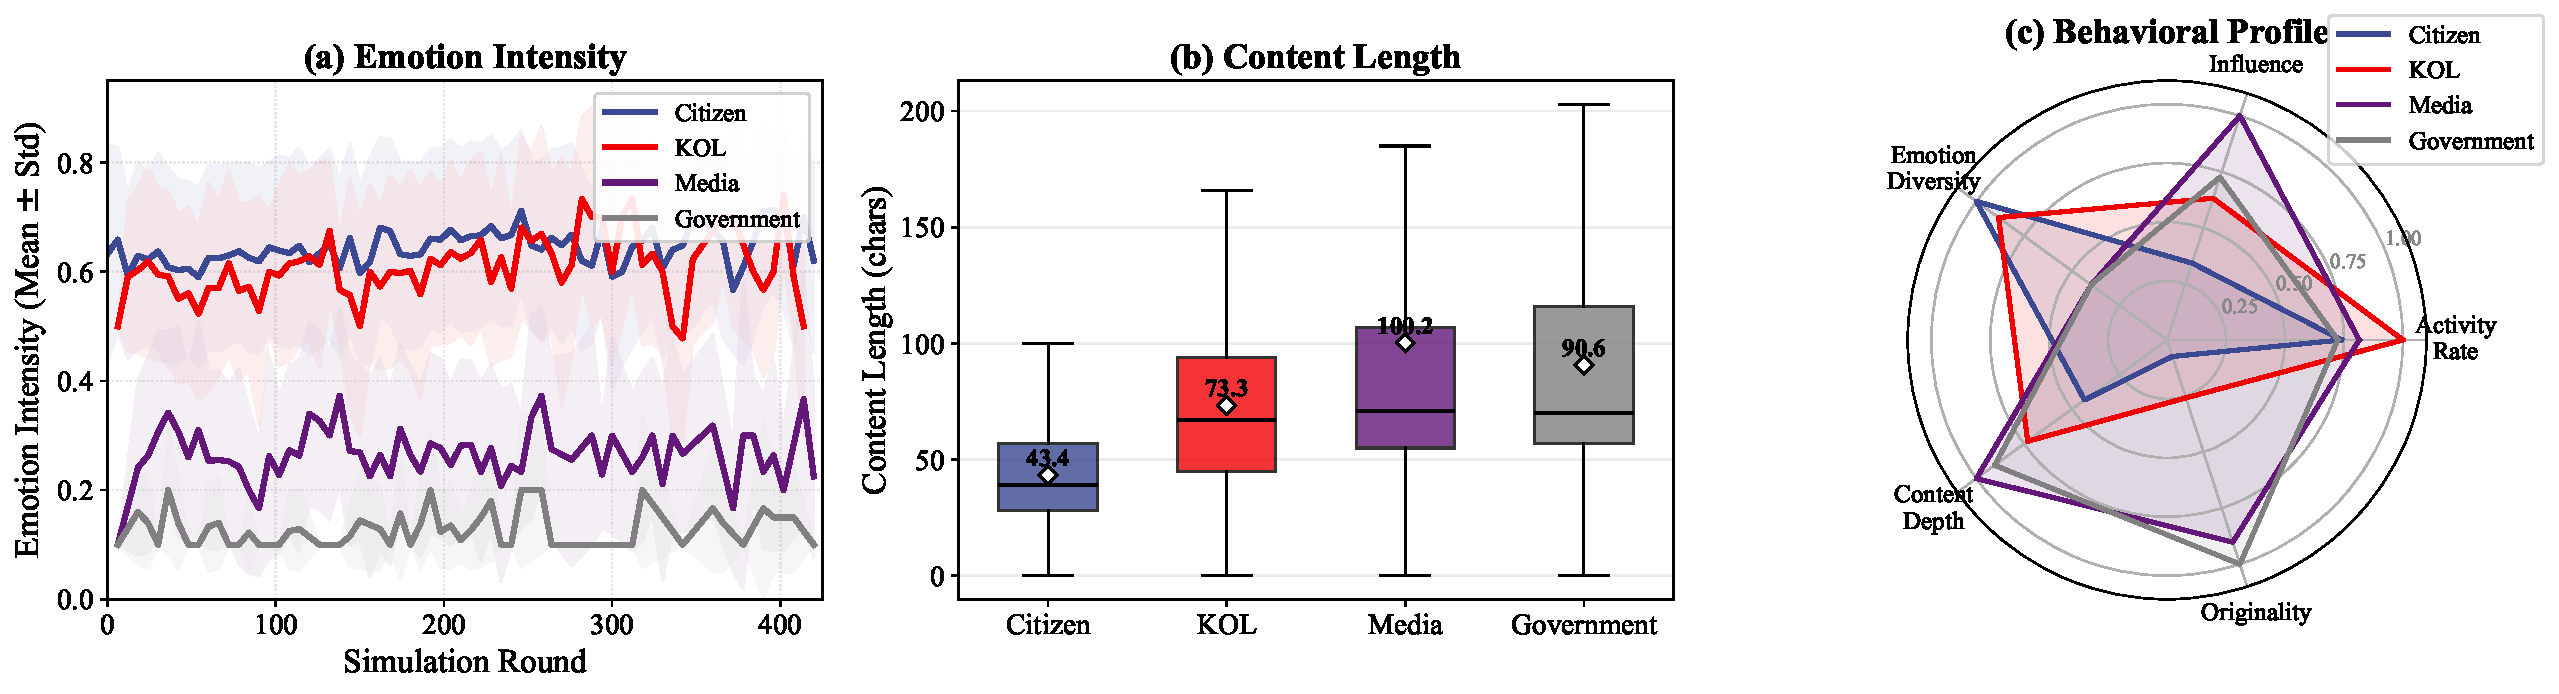
\includegraphics[width=\columnwidth]{fig_paper_heterogeneity.pdf}
\caption{四类智能体行为异质性。(a)~情绪强度时序演化；(b)~内容长度分布；(c)~多维行为特征雷达图。}
\label{fig:heterogeneity}
\end{figure}

图~\ref{fig:heterogeneity}从情绪强度、内容长度和多维行为画像三个角度展示了四类智能体涌现出的系统性异质性。在情绪强度维度上，Citizen和KOL的平均情绪强度分别为0.645和0.603，始终处于高唤醒区间，且在事件刺激后呈现更剧烈的波动；Media和Government则稳定在低唤醒区间，呈现公众情绪化、官方中性化的分层模式，与真实舆情中“大众愤怒、官媒克制”的普遍观察一致。在内容长度维度上，Media和Government智能体的平均内容长度显著高于Citizen，反映了官方和媒体智能体生成更为详尽、结构化的内容输出。雷达图上四类智能体形成了形态截然不同的多边形，Citizen在情绪维度和互动频率上突出，KOL在影响力和内容产出量上领先，Media在内容质量和中性表达上占优，Government则以低频但高权威性的发言为特征。这些异质性模式并非手动编码，而是由Social-BDI架构中差异化的角色信念和动机权重自然涌现，验证了框架在多主体异质性建模上的有效性。

\subsubsection{情绪唤醒与极化效应}

基于情绪唤醒理论~\citep{berger_what_2012}和情绪传染假说~\citep{hatfield_emotional_1994}，我们从唤醒自增强和情绪传染两个维度进行验证（表~\ref{tab:emotion}）。唤醒自增强维度包含三个指标：（1）\textit{高唤醒趋势系数}$\beta$，通过对高唤醒情绪（如愤怒、兴奋等强刺激情绪）占比进行线性回归拟合获得，$\beta>0$表明高唤醒情绪随时间推进呈上升趋势；（2）\textit{高唤醒情绪占比}，统计仿真全过程中高唤醒情绪在所有情绪表达中的比例，用于验证高唤醒情绪是否在舆情讨论中占据主导地位；（3）\textit{高/低唤醒强度比}，计算高唤醒情绪的平均强度与低唤醒情绪平均强度之比，反映两类情绪在表达力度上的差异。情绪传染维度包含两个指标：（4）\textit{评论链情绪一致率}，计算每条评论链中相邻评论之间情绪极性一致的比例，高一致率表明上游情绪对下游评论产生了传染效应；（5）\textit{升级/降级比}，统计情绪从低唤醒转向高唤醒（升级）与从高唤醒转向低唤醒（降级）的次数之比，该比值大于1表明情绪在互动中更倾向于持续强化而非回落，呈现棘轮式累积特征。

\begin{table}[!t]
\centering
\caption{Emotional arousal theory validation metrics.}
\label{tab:emotion}
\renewcommand{\arraystretch}{1.0}
\resizebox{\columnwidth}{!}{%
\scriptsize
\begin{tabular}{@{}p{1.5cm}p{3.0cm}cc@{}}
\toprule
\textbf{Dimension} & \textbf{Metric} & \textbf{Sim.\ Result} & \textbf{Theoretical Expectation} \\
\midrule
\multirow{3}{1.5cm}{Arousal Self-Reinforcement$^{\rm a}$}
 & High-arousal trend coeff.\ $\beta$ & $3.41{\times}10^{-4}$\,($p{<}.001$) & $\beta > 0$ \\
 & High-arousal emotion ratio & 73.5\% & Dominant \\
 & High/low arousal intensity ratio & 2.0$\times$ & $>1$ \\
\midrule
\multirow{2}{1.5cm}{Emotional Contagion$^{\rm b}$}
 & Comment-chain emotion consistency & 0.772 & $\gg$ random baseline \\
 & Escalation/de-escalation ratio & 4.78 & $>1$ (ratchet effect) \\
\bottomrule
\end{tabular}%
}
\vspace{3pt}
{\footnotesize $^{\rm a}$~\citet{berger_what_2012};\quad $^{\rm b}$~\citet{hatfield_emotional_1994}}
\end{table}

高唤醒情绪通常指具有较强刺激性和兴奋性的情绪状态。仿真结果显示，此类情绪的占比随过程推进呈显著上升趋势，最终达到73.5\%，这与已有研究关于高唤醒情绪更易促进内容分享与传播的结论一致~\citep{berger_what_2012}。与此同时，评论链的情绪一致率高达0.772；进一步比较情绪由低唤醒向高唤醒转变的次数与由高唤醒向低唤醒转变的次数，二者比值达到4.78，表明情绪在互动过程中更倾向于持续强化而非回落，呈现出明显的棘轮式累积特征，从而为情绪传染假说提供了支持~\citep{hatfield_emotional_1994}。
进一步地，我们定义极化指数$\text{PI} = 1 - H/H_{\max}$。如图~\ref{fig:polarization}所示，极化指数从早期的0.41攀升至晚期的0.67（升幅63\%，$p < 0.001$），表明系统中的情绪分布随仿真推进不断向少数主导情绪集中，这一演化趋势与回音室环境下情绪趋同和强化的理论预期相一致~\citep{cinelli_echo_2021}。

\begin{figure}[!t]
\centering
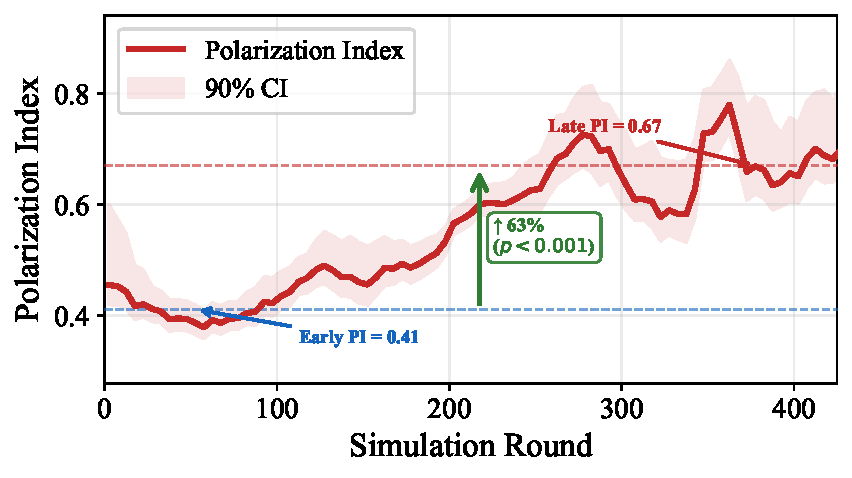
\includegraphics[width=0.85\columnwidth]{fig_paper_polarization.pdf}
\caption{情绪极化指数（PI）随仿真轮次的演化。实线为PI均值，阴影为90\% Bootstrap置信区间，虚线标注早期与晚期均值。}
\label{fig:polarization}
\end{figure}

\subsubsection{无标度拓扑与级联幂律}

\begin{figure}[!t]
\centering
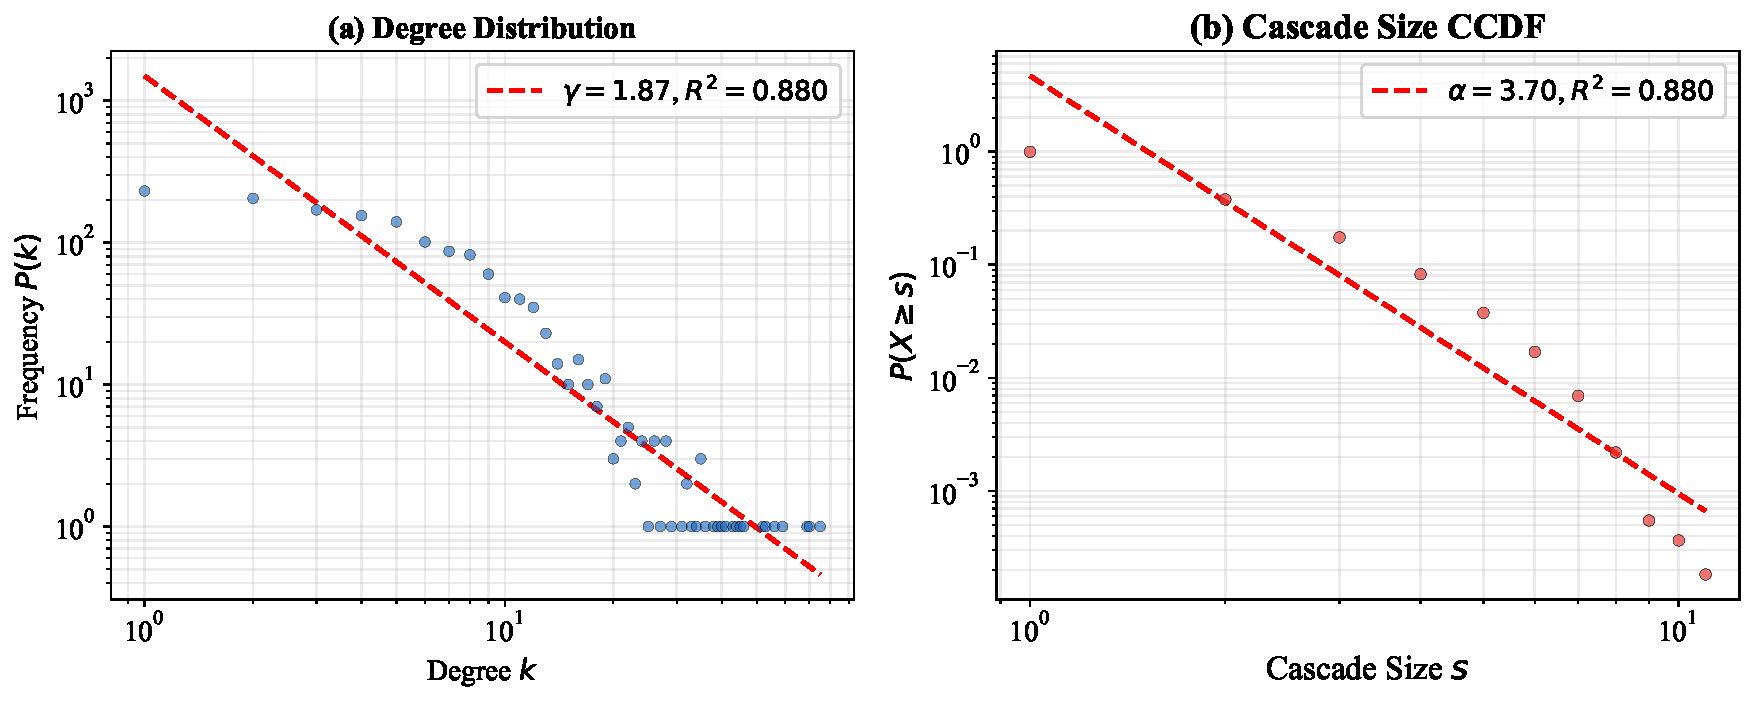
\includegraphics[width=\columnwidth]{fig_paper_powerlaw.pdf}
\caption{互动网络的拓扑特性。(a)~度分布幂律拟合$P(k) \sim k^{-\gamma}$；(b)~级联规模CCDF$P(X \geq s) \sim s^{-\alpha}$。}
\label{fig:powerlaw}
\end{figure}

真实社交网络的度分布和信息级联规模普遍服从幂律分布~\citep{barabasi_albert_1999}。如图~\ref{fig:powerlaw}(a)所示，互动网络的度分布幂律拟合指数$\gamma = 1.87$（$R^2 = 0.880$），落在真实社交网络中普遍报告的$1.5 < \gamma < 3$范围内，表明仿真网络呈现出典型的无标度特征，即少数意见领袖节点形成高度数枢纽，而大量普通用户仅有少量连接。如图~\ref{fig:powerlaw}(b)所示，信息级联规模的互补累积分布函数（CCDF）拟合$\alpha = 3.70$（$R^2 = 0.880$），表明仿真中绝大多数转发级联规模较小，但偶尔出现涉及大量用户的爆发性传播，这与真实微博中“多数帖子无人问津、少数帖子病毒传播”的长尾现象一致。

\subsection{统计结果校准}\label{subsec:stat}

本节将仿真输出与三个真实舆情事件进行直接对比，从\textbf{行为层}（行为类型分布与活跃度曲线）、\textbf{内容层}（话语非理性、词汇多样性与情感倾向）和\textbf{拓扑层}（网络结构与信息级联）三个维度进行系统性校准。

\subsubsection{对比方法}

统计校准关注大规模多智能体交互后涌现的群体行为是否在统计意义上与真实数据一致，因此对比方法需要在完整的仿真环境中运行端到端的多步仿真。设置三种对比基线：\textbf{Rule-based ABM}采用传统的规则驱动仿真，每个智能体根据其所属角色类型（普通用户、意见领袖、媒体、政府）预定义的行为概率分布进行随机采样，以确定当前时间步执行的行为类型（如发帖、评论、转发等），整个决策过程完全基于预设规则，不涉及任何LLM调用。\textbf{POSIM w/ LLM}在POSIM仿真环境下移除Social-BDI认知架构，智能体在接收推荐内容后直接由LLM单步生成行为决策和内容，不进行显式的信念更新或欲望推理。\textbf{POSIM w/ CoT}将Social-BDI的三阶段独立模块替换为单次思维链推理，在同一LLM调用中串联完成从认知到行为的全过程，保留POSIM的其他一切模式。

\subsubsection{评估指标}

评估从行为、内容和拓扑三个层面对仿真输出与真实数据进行定量比对，共计九个指标。

\textbf{行为层}度量智能体群体行为模式与真实用户的一致性，包含三个指标。行为类型分布散度BType JSD采用Jensen-Shannon散度衡量模拟与真实行为类型概率分布的差异，定义为：
\begin{equation}
\text{JSD}(P \| Q) = \tfrac{1}{2} D_{\text{KL}}(P \| M) + \tfrac{1}{2} D_{\text{KL}}(Q \| M)
\end{equation}
其中$M = (P + Q)/2$为两分布的均值分布。活跃度曲线Pearson相关系数Act.\,$\rho$衡量模拟与真实活跃度时序的线性相关性，活跃度曲线均方根误差Act.\,RMSE衡量两条曲线的逐点均方根偏差。

\textbf{内容层}度量生成文本的语义特征与真实内容的匹配程度，包含三个指标。话语非理性相似度Irrat.\,Sim.基于关键词将话语分为非理性、理性和中立三类，计算模拟与真实分布的相似度；该指标直接反映仿真系统能否再现真实舆情中由情绪驱动、认知偏差主导的非理性话语格局，而这正是Social-BDI架构中信念模块对行为激发的核心体现。词汇多样性偏差$|\Delta\text{TTR}|$衡量模拟与真实文本词汇丰富度的差异，其中TTR为Type-Token Ratio。情感均值偏差$|\Delta\bar{S}|$衡量真实群体情感均值与模拟均值的整体偏移，其中$S$为基于情感分析模型库SnowNLP输出的情感得分（正值表示正面情感，负值表示负面情感）。

\textbf{拓扑层}度量仿真中涌现的网络结构与传播模式，包含三个指标。网络结构相似度Net.\,Sim.比较模拟与真实互动网络的拓扑特征，级联规模分布相似度Casc.\,Sim.比较信息级联规模的统计分布，级联幂律相似度Casc.\,PL比较级联规模幂律拟合参数的接近程度。

各层内的平均得分通过对越小越优的指标取$1{-}x$归一化后与越大越优的指标共同求均值得到。

\subsubsection{校准结果}

\begin{table*}[!t]
\centering
\caption{Statistical calibration results across three events (LE\,=\,Luxury Earring, WL\,=\,WHU Library, XF\,=\,Xibei Prepared Food). \textbf{Bold}: best per dataset; \na: not applicable. \textcolor{gaingreen}{Green}: gain of POSIM over the second-best method.}
\label{tab:calibration}
\vspace{2pt}
\renewcommand{\arraystretch}{1.05}
\resizebox{\textwidth}{!}{%
\footnotesize
\begin{tabular}{@{}cl cccc cccc cccc@{}}
\toprule
\multirow{2}{*}{\textbf{Data}} & \multirow{2}{*}{\textbf{Method}}
& \multicolumn{4}{c}{\textbf{Behavior Layer}}
& \multicolumn{4}{c}{\textbf{Content Layer}}
& \multicolumn{4}{c}{\textbf{Topology Layer}} \\
\cmidrule(lr){3-6} \cmidrule(lr){7-10} \cmidrule(lr){11-14}
& & \makecell{BType\\JSD\,$\downarrow$} & \makecell{Act.\\$\rho$\,$\uparrow$} & \makecell{Act.\\RMSE\,$\downarrow$} & \makecell{Avg.\\$\uparrow$}
& \makecell{Irrat.\\Sim.\,$\uparrow$} & \makecell{$|\Delta\text{TTR}|$\\$\downarrow$} & \makecell{$|\Delta\bar{S}|$\\$\downarrow$} & \makecell{Avg.\\$\uparrow$}
& \makecell{Net.\\Sim.\,$\uparrow$} & \makecell{Casc.\\Sim.\,$\uparrow$} & \makecell{Casc.\\PL\,$\uparrow$} & \makecell{Avg.\\$\uparrow$} \\
\midrule
\multirow{5}{*}{\textbf{LE}}
& Rule-based ABM        & 0.427 & 0.808 & 0.158 & 0.741 & \na & \na & \na & \na & 0.479 & 0.633 & 0.543 & 0.552 \\
& POSIM w/ LLM        & 0.289 & 0.799 & 0.162 & 0.783 & 0.544 & 0.185 & 0.319 & 0.680 & 0.565 & 0.735 & 0.918 & 0.739 \\
& POSIM w/ CoT          & 0.394 & 0.806 & \best{0.151} & 0.754 & 0.584 & 0.141 & 0.123 & 0.774 & 0.755 & 0.777 & 0.756 & 0.763 \\
\rowcolor{oursrow}
& \textbf{POSIM (Ours)}  & \best{0.193} & \best{0.809} & 0.154 & \best{0.821} & \best{0.790} & \best{0.030} & \best{0.029} & \best{0.910} & \best{0.895} & \best{0.830} & \best{0.961} & \best{0.896} \\[1pt]
\rowcolor{oursrow}
& \textit{Improvement} & \gain{+.096} & \gain{+.001} & \gain{+.000} & \gain{+.038} & \gain{+.206} & \gain{+.111} & \gain{+.094} & \gain{+.136} & \gain{+.140} & \gain{+.053} & \gain{+.043} & \gain{+.133} \\
\midrule
\multirow{5}{*}{\textbf{WL}}
& Rule-based ABM        & 0.318 & 0.681 & 0.126 & 0.746 & \na & \na & \na & \na & 0.869 & 0.696 & 0.642 & 0.736 \\
& POSIM w/ LLM        & 0.237 & 0.722 & 0.119 & 0.789 & 0.453 & 0.172 & 0.360 & 0.640 & 0.528 & 0.667 & 0.580 & 0.592 \\
& POSIM w/ CoT          & 0.229 & 0.744 & \best{0.116} & 0.800 & 0.474 & 0.091 & 0.365 & 0.673 & \best{0.941} & 0.740 & 0.673 & 0.784 \\
\rowcolor{oursrow}
& \textbf{POSIM (Ours)}  & \best{0.073} & \best{0.750} & 0.118 & \best{0.853} & \best{0.841} & \best{0.010} & \best{0.203} & \best{0.876} & 0.850 & \best{0.758} & \best{0.965} & \best{0.858} \\[1pt]
\rowcolor{oursrow}
& \textit{Improvement} & \gain{+.156} & \gain{+.006} & \gain{+.000} & \gain{+.053} & \gain{+.367} & \gain{+.081} & \gain{+.157} & \gain{+.203} & \gain{+.000} & \gain{+.018} & \gain{+.292} & \gain{+.074} \\
\midrule
\multirow{5}{*}{\textbf{XF}}
& Rule-based ABM        & 0.312 & 0.664 & 0.187 & 0.721 & \na & \na & \na & \na & 0.528 & 0.614 & 0.279 & 0.474 \\
& POSIM w/ LLM        & 0.244 & 0.671 & 0.190 & 0.746 & 0.765 & 0.117 & 0.076 & 0.858 & 0.774 & 0.695 & 0.482 & 0.650 \\
& POSIM w/ CoT          & 0.293 & 0.699 & 0.181 & 0.742 & 0.774 & 0.134 & \best{0.014} & 0.875 & 0.767 & 0.696 & 0.460 & 0.641 \\
\rowcolor{oursrow}
& \textbf{POSIM (Ours)}  & \best{0.148} & \best{0.727} & \best{0.168} & \best{0.804} & \best{0.843} & \best{0.019} & 0.046 & \best{0.926} & \best{0.885} & 0.696 & \best{0.513} & \best{0.698} \\[1pt]
\rowcolor{oursrow}
& \textit{Improvement} & \gain{+.096} & \gain{+.028} & \gain{+.013} & \gain{+.058} & \gain{+.069} & \gain{+.098} & \gain{+.000} & \gain{+.051} & \gain{+.111} & \gain{+.000} & \gain{+.031} & \gain{+.048} \\
\bottomrule
\end{tabular}%
}
\end{table*}

实验在三个真实舆情数据集上开展，结果如表~\ref{tab:calibration}所示（三个事件的统计校准可视化详见附录图~\ref{fig:three_event_calibration}）。

\textbf{行为层校准。}POSIM在三个数据集上的BType JSD均取得最优，说明Social-BDI架构产生的行为决策在类型比例上与真实数据高度一致。值得注意的是，WL数据集的JSD仅为0.073，远优于其他方法，这与该事件中校园讨论的行为模式相对集中有关，Social-BDI的信念锚定机制使智能体能够准确捕捉这种集中趋势。仅使用LLM单步决策（POSIM w/ LLM）时，行为分布偏差显著增大，尤其在LE和XF数据集上JSD分别达到0.289和0.244，表明缺乏分层认知约束的LLM倾向于产生行为类型趋同。热度时序相关性$\rho$方面，POSIM在三个数据集上均保持高相关度，表明霍克斯点过程驱动的时间引擎有效捕捉了舆情活跃度的时序波动模式。行为层平均得分在三个数据集上分别达到0.821、0.853和0.804，跨事件类型的稳定表现证明了框架的通用性。

\textbf{内容层校准。}POSIM的非理性相似度在所有数据集上均最高，表明Social-BDI架构能够准确再现舆情中理性与非理性话语的分布格局。这一优势得益于信念子系统对情绪激发与认知偏差的显式建模，使智能体能够在信念状态驱动下生成符合其认知状态的非理性表达。相比之下，POSIM w/ LLM的非理性相似度较低，差距在LE数据集上尤为显著（0.790 vs. 0.544），原因在于天价耳环事件中公众非理性情绪强烈，缺乏信念模块的认知驱动使LLM生成的内容倾向于中性化表达，无法再现真实舆情中的非理性话语格局。词汇多样性差异$|\Delta\text{TTR}|$在所有数据集上同样最小，表明分层认知推理中信念模块维护的个性化角色信息有效避免了LLM的平均人格问题，使不同智能体产生了具有个人风格的差异化文本。情感偏差$|\Delta\bar{S}|$方面，POSIM在所有数据集上均保持极低水平，说明Social-BDI中情绪因素的显式建模使仿真内容的整体情感倾向与真实数据高度吻合。内容层平均得分在三个数据集上分别为0.910、0.876和0.926。

\textbf{拓扑层校准。}评估采用内容来源链追踪机制，POSIM在三个数据集上均取得最优的拓扑层平均得分。在网络相似度维度上，POSIM在LE和XF数据集上分别达到0.895和0.885，显著优于Rule-based ABM的0.479和0.528，表明Social-BDI的多级意图规划使智能体能够基于内容质量和社交亲和度做出有区分度的交互选择，从而涌现出更接近真实的网络拓扑。在级联幂律维度上，差异更为显著，POSIM在LE数据集上达到0.961，而Rule-based ABM仅为0.543，说明随机交互决策无法产生真实社交网络中的长尾级联分布。XF数据集的拓扑层平均得分相对较低，可能与该事件持续时间较长、网络结构更为复杂有关，但POSIM仍显著优于所有基线方法。

\textbf{综合分析。}POSIM在三个层面均全面领先，核心优势源于Social-BDI架构的分层认知设计：信念子系统为行为决策提供个性化的认知锚定，欲望子系统通过动机约束驱动非理性话语的准确再现，意图子系统的结构化分解保障了词汇多样性和交互拓扑的合理性。三个基线的表现差异也佐证了这一判断——Rule-based ABM因缺乏认知驱动而在多数数据集的拓扑层表现较差，POSIM w/ LLM因缺少信念锚定而在内容层一致性不足，POSIM w/ CoT因模块间缺乏独立约束而整体居中。

\vspace{6pt}
\subsection{消融实验}

为验证POSIM各核心模块的必要性，设置完整框架与若干变体配置进行对比。\textbf{Full POSIM}为包含所有模块的完整框架。\textbf{w/o Belief}移除信念更新模块，智能体不维护显式的信念状态，欲望和意图直接基于当前感知信息生成，不参考历史认知积累。\textbf{w/o Desire}移除欲望生成模块，意图规划不再接收动机权重约束，LLM直接从信念状态生成行为决策，缺失了动机层面的中间推理。\textbf{w/o Intention}移除意图规划模块，行为决策不再经过三级思维链的结构化分解（行为选择、表达策略规划和内容生成），LLM直接从信念和欲望状态生成最终行为输出，缺失了表达策略层面的显式约束。\textbf{w/o Hawkes}将霍克斯点过程时间引擎替换为固定时间步长的均匀激活模式，每步激活固定数量的智能体，移除了事件驱动的动态时间调度机制。结果如表~\ref{tab:ablation}所示。

\begin{table}[!t]
\centering
\caption{Ablation study results (LE dataset). \underline{Underline} marks cases where a variant outperforms the full model.}
\label{tab:ablation}
\renewcommand{\arraystretch}{1.0}
\resizebox{\columnwidth}{!}{%
\scriptsize
\begin{tabular}{@{}l ccc ccc cc@{}}
\toprule
\multirow{2}{*}{\textbf{Configuration}} & \multicolumn{3}{c}{\textbf{Behavior Layer}} & \multicolumn{3}{c}{\textbf{Content Layer}} & \multicolumn{2}{c}{\textbf{Topology Layer}} \\
\cmidrule(lr){2-4} \cmidrule(lr){5-7} \cmidrule(lr){8-9}
& \makecell{JSD\\$\downarrow$} & \makecell{$\rho$\\$\uparrow$} & \makecell{RMSE\\$\downarrow$}
& \makecell{Irrat.\\$\uparrow$} & \makecell{$|\Delta$TTR$|$\\$\downarrow$} & \makecell{$|\Delta\bar{S}|$\\$\downarrow$}
& \makecell{Net.\\$\uparrow$} & \makecell{Casc.\\$\uparrow$} \\
\midrule
\rowcolor{grayrow}
Full POSIM & \best{0.193} & \best{0.809} & \best{0.154} & \best{0.790} & \best{0.030} & \best{0.029} & \best{0.895} & \best{0.830} \\
w/o Belief & 0.258 & 0.762 & 0.172 & 0.706 & 0.058 & 0.067 & 0.861 & 0.773 \\
w/o Desire & 0.267 & 0.779 & 0.169 & 0.682 & 0.071 & 0.083 & 0.853 & 0.788 \\
w/o Intention & 0.237 & 0.802 & 0.159 & 0.728 & 0.064 & 0.055 & 0.858 & 0.814 \\
w/o Hawkes & \underline{0.177} & 0.235 & 0.362 & 0.787 & 0.207 & \underline{0.028} & 0.822 & 0.754 \\
\bottomrule
\end{tabular}%
}
\end{table}

\textbf{w/o Hawkes}移除霍克斯点过程后，$\rho$从0.809骤降至0.235，RMSE从0.154恶化至0.362，表明均匀激活模式无法捕捉舆情活跃度的时序波动。其BType JSD（0.177）略优于Full POSIM（0.193），这是因为均匀激活使每步采样的智能体数量保持恒定，在大量均匀采样下行为类型比例更容易收敛至其内在概率均值，从而在分布层面偶然接近真实数据，但这一微弱优势以丧失事件驱动的活跃度突变特征为代价。$|\Delta\text{TTR}|$恶化至0.207，说明时间引擎异常间接导致内容同质化。

\textbf{w/o Belief}移除信念模块后各指标普遍下降：JSD恶化至0.258，非理性相似度从0.790降至0.706，$|\Delta\bar{S}|$恶化至0.067。信念模块维护的$B^{evt}$和$B^{emo}$是驱动非理性话语生成的核心依据，其缺失导致智能体丧失对争议焦点的深层认知与情绪激发。

\textbf{w/o Desire}移除欲望模块后内容层退化最严重：非理性相似度降至0.682（所有变体最低），$|\Delta\bar{S}|$恶化至0.083（最大），表明动机类型是驱动非理性话语表达的核心因素，缺失后LLM倾向于生成中性化文本。

\textbf{w/o Intention}移除意图模块后，$|\Delta\text{TTR}|$恶化至0.064，网络相似度下降3.7pp，表明三级思维链的结构化分解对词汇多样性和交互拓扑具有重要贡献。

\textbf{综合分析。}四组消融实验表明各组件具有清晰的功能分工，其中信念子系统提供全局认知支撑，欲望子系统驱动内容层的非理性表达，意图子系统保障词汇多样性和交互拓扑，霍克斯引擎决定时序一致性，验证了Social-BDI分层架构各组件的互补性。

% ============================================================
% 第6节 讨论（原第5节，因插入第4节验证框架后顺延）
% ============================================================
\section{讨论}\label{sec:discussion}

本节首先通过两项案例研究展示POSIM作为计算实验平台的应用价值，随后总结主要发现并讨论局限性。

\subsection{认知引导实验}

基于天价耳环事件设计认知引导实验，我们选择了仿真过程中某个事件点爆发后的某个时间步开始，然后直接修改智能体心理认知信念的部分条目，从而达到模拟并观察不同认知倾向人群对事件响应的效果，分别测试30\%、60\%和100\%三种覆盖率。对照组保持无干预基线，三种干预策略分别对应不同的认知调控机制。\textbf{理性认知引导}（RC）引导智能体从多角度理性分析事件，\textbf{共情引导}（EP）鼓励理解当事人立场，\textbf{情绪调节}（ER）引导智能体识别和管理自身情绪。结果如表~\ref{tab:priming}所示。

\begin{table}[!t]
\centering
\caption{Cognitive priming experiment results. Coverage denotes the proportion of agents receiving cognitive priming.}
\label{tab:priming}
\scriptsize
\renewcommand{\arraystretch}{1.0}
\begin{tabular}{@{}llccc@{}}
\toprule
\textbf{Condition} & \textbf{Coverage} & \makecell{\textbf{Neg.\ Emotion}\\\textbf{Ratio}\,$\downarrow$} & \makecell{\textbf{Anger}\\\textbf{Ratio}\,$\downarrow$} & \makecell{\textbf{Emotion}\\\textbf{Intensity}\,$\downarrow$} \\
\midrule
Control & --- & 0.844 & 0.600 & 0.649 \\
\midrule
 & 30\% & 0.767 & 0.534 & 0.621 \\
 & 60\% & 0.753 & 0.506 & 0.595 \\
\rowcolor{grayrow}
\multirow{-3}{*}{\makecell[l]{Rational\\Cognition (RC)}} & 100\% & \best{0.571} & \best{0.407} & \best{0.527} \\
\midrule
\multirow{3}{*}{\makecell[l]{Empathy\\Priming (EP)}}
 & 30\% & 0.794 & 0.523 & 0.609 \\
 & 60\% & 0.806 & 0.535 & 0.617 \\
 & 100\% & 0.878 & 0.569 & 0.650 \\
\midrule
\multirow{3}{*}{\makecell[l]{Emotional\\Regulation (ER)}}
 & 30\% & 0.831 & 0.583 & 0.626 \\
 & 60\% & 0.644 & 0.503 & 0.587 \\
 & 100\% & 0.572 & 0.481 & 0.573 \\
\bottomrule
\end{tabular}
\end{table}

实验揭示了以下关键发现。首先，RC和ER策略均显著降低负面情绪比例（Negative Emotion Ratio, NER），且呈现剂量效应。如表~\ref{tab:priming}所示，RC将NER从0.844降至0.571（降幅32.3\%），整体情绪强度也明显下降；RC的覆盖率跨越60\%后效果显著跃升，呈现阈值效应。ER策略同样表现出显著的剂量效应，100\%覆盖时NER降至0.572，与RC的效果接近，揭示了感受层调控与认知层引导在情绪缓解上的互补性。

\textbf{共情悖论效应。}实验中最具理论价值的发现来自共情引导（EP）策略。社会心理学研究表明，共情在理解他人痛苦的同时会诱发观察者自身的移情性负面情绪（empathic distress），在特定条件下反而可能加剧负面情绪扩散~\citep{batson_empathy_1991}。本实验中，EP策略的负面情绪比例达0.878，高于对照组的0.844，且随覆盖率从30\%增至100\%呈单调上升，表现出与RC和ER截然相反的反剂量效应。从机制层面分析，共情引导通过修改心理认知信念（$B^{psy}$）增强了智能体对他人情绪的敏感性，使其在信念更新中更强烈地吸收负面情感色彩，并经由情绪传染机制在社交网络中形成正反馈回路，最终加速了移情性负面情绪的级联传播。Social-BDI的分层认知架构使这一从认知信念改变到情绪状态变化再到社交传染放大的完整因果链条可追溯、可解释。

这一发现表明，基于LLM的多智能体仿真系统已具备涌现复杂社会心理现象的能力，可作为社会科学理论的计算实验平台。在实践层面，共情悖论的定量观察为舆情治理提供了直接警示，旨在缓和群体对立的共情引导策略在负面情绪主导的舆论场中可能适得其反，治理者应优先采用理性认知引导或情绪调节等直接作用于认知层或感受层的策略。

\begin{figure}[!t]
\centering
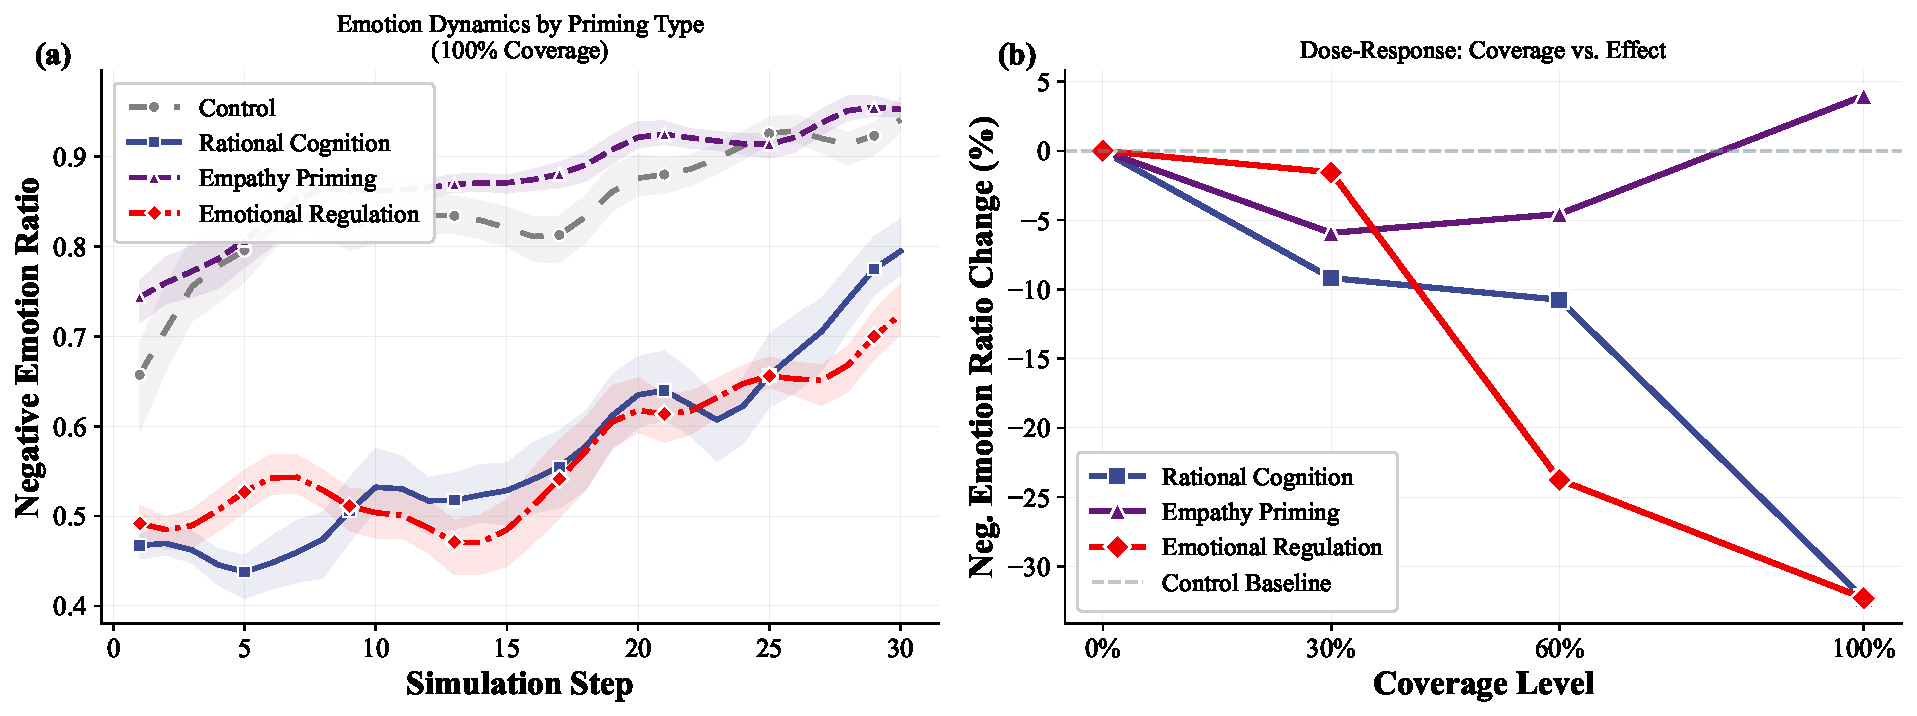
\includegraphics[width=\columnwidth]{paper_cognitive_priming.pdf}
\caption{Empathy paradox experimental results. (a) Emotional arousal evolution under two strategies: the empathy-based guidance (dashed) yields persistently higher arousal than the baseline (solid) from the mid-stage onward. (b) Behavioral distribution comparison: empathy-based guidance produces higher proportions of emotionally intense behavior categories (short comments, reposts with comment). (c) Discourse irrationality comparison: the empathy-guided group exhibits a higher proportion of irrational discourse.}
\label{fig:cognitive_priming}
\end{figure}

\subsection{反事实策略评估}

基于西贝预制菜事件设计反事实实验，保持外部事件不变，仅替换西贝的公关响应，比较五种策略。\textbf{实际应对}（AR）复现了西贝从强硬否认到辱骂再到秒删致歉的真实应对过程，\textbf{及时致歉}（SEA）在事件初期即发布诚恳致歉声明，\textbf{主动透明}（PT）主动公开预制菜使用信息和食品安全报告，\textbf{消费者对话}（CD）直接与消费者进行互动和沟通，\textbf{战略沉默}（SS）对事件不做任何公开回应。结果见表~\ref{tab:counter}。

\begin{table}[!t]
\centering
\caption{Counterfactual strategy evaluation results.}
\label{tab:counter}
\scriptsize
\renewcommand{\arraystretch}{1.0}
\begin{tabular}{@{}lp{1.5cm}p{1.2cm}p{1.5cm}@{}}
\toprule
\textbf{Strategy} & \makecell{\textbf{Neg.\ Emotion}\\\textbf{Ratio}\,$\downarrow$} & \makecell{\textbf{Anger}\\\textbf{Ratio}\,$\downarrow$} & \makecell{\textbf{Emotion}\\\textbf{Intensity}\,$\downarrow$} \\
\midrule
Actual Response (AR) & 0.792 & 0.685 & 0.685 \\
Swift Early Apology (SEA) & 0.749 & 0.621 & 0.612 \\
Proactive Transparency (PT) & 0.773 & 0.658 & 0.645 \\
\rowcolor{grayrow}
Consumer Dialogue (CD) & \best{0.744} & \best{0.612} & \best{0.598} \\
Strategic Silence (SS) & 0.831 & 0.714 & 0.702 \\
\bottomrule
\end{tabular}
\end{table}

实验揭示了以下关键发现。积极策略显著优于消极应对，CD策略效果最优（NER为0.744），SEA次之（0.749），PT第三（0.773）。战略沉默表现最差（NER达0.831），其情绪强度甚至高于实际应对，验证了危机公关中沉默并非最优选择的教训。策略传导严格遵循信念修正、认知推理改变、行为输出转变的因果链条，验证了Social-BDI架构在策略评估中的可解释性优势。

\subsection{主要发现}

可信验证体系的实验结果支撑了以下发现。在微观层面，Social-BDI架构在认知行为链一致性（4.64/5.0）、人格稳定性（0.661）和决策抗扰性（0.695）上全面优于基线方法，验证了分层认知建模相较于端到端生成的系统性优势。值得注意的是，CoT方法的决策抗扰性反而最低（0.541），表明单次调用中串联的认知推理缺乏稳定的状态锚定，而Social-BDI通过独立模块化的显式信念状态提供了认知锚定效应。在宏观层面，仿真系统在无显式宏观编程的条件下自发涌现出舆情生命周期、行为异质性、情绪极化（极化指数从0.41升至0.67）、无标度拓扑（$\gamma=1.87$）和级联幂律分布（$\alpha=3.70$）等与社会科学理论一致的集体行为模式。在统计校准层面，POSIM在三个数据集上全面优于基线方法，行为、内容和拓扑指标分别提升\textbf{5.0\%}、\textbf{13.0\%}和\textbf{8.5\%}。消融实验表明各认知子系统功能互补，欲望子系统对非理性话语再现贡献最显著，信念子系统为个性化决策提供不可替代的认知锚定。

\subsection{局限性}

尽管实验结果整体积极，本研究仍存在若干不足。首先，框架的认知推理质量与底层LLM的能力紧密耦合，大规模仿真的推理成本也仍有压缩空间。其次，当前社交网络中的关注关系在仿真过程中保持静态，尚未纳入用户间关注与取关的动态演化机制。再者，实验验证仅覆盖微博平台，框架在不同社交媒体平台和文化语境下的迁移能力有待进一步考察。此外，基于大模型的仿真技术向来存在巨大的资源消耗问题，本文也面临类似挑战，未来如何在token消耗和仿真性能之间进行平衡将是研究重点。

% ============================================================
% 第7节 结论（原第6节）
% ============================================================
\section{结论}\label{sec:conclusion}

“\textit{All models are wrong, but some are useful.}”~\citep{box_draper_1987_emprical_modelbuilding}舆情仿真研究的关键不在于追求对现实的逐点复刻，而在于获得对舆情机制与演化规律\textbf{足够可信且可用于决策}的近似。本文提出了社交媒体舆情仿真框架POSIM，其核心思路是将大语言模型嵌入Social-BDI分层认知架构以构建具有显式认知状态的智能体，并以霍克斯自激点过程统一建模外生事件冲击与内生用户交互，从而在分钟级时间分辨率下实现高精度的舆情演化仿真。

三层递进的可信验证结果支撑了以下结论。在微观层面，Social-BDI架构在认知行为链一致性、人格稳定性和决策抗扰性上全面优于直接提示与思维链方法，证实了分层独立认知建模相较于端到端生成的系统性优势。在宏观层面，仿真系统在无显式宏观编程的条件下自发涌现出舆情生命周期、情绪极化、无标度拓扑和级联幂律等与社会科学理论一致的集体行为模式。在统计校准层面，POSIM的行为、内容和拓扑指标相较于最优基线分别提升了5.0\%、13.0\%和8.5\%，跨事件类型的稳健表现验证了框架的通用性。此外，两项案例研究展示了框架向认知干预和反事实策略评估等应用场景扩展的能力，表明POSIM不仅是一个社会实验仿真器，更具备作为舆情治理计算实验平台的潜力。

% ============================================================
% 参考文献
% ============================================================
\bibliographystyle{model5-names}
\bibliography{posim_refs}

% ============================================================
% 附录
% ============================================================
\appendix

% ============================================================
% 附录A：核心算法伪代码
% ============================================================
\section{核心算法伪代码}

\noindent
\begin{minipage}[t]{\columnwidth}
\begin{algorithm}[H]
\caption{POSIM仿真主循环}
\label{alg:main}
\begin{algorithmic}[1]
\REQUIRE 智能体集合$\mathcal{U}$，事件队列$\mathcal{E}$，配置$\mathcal{C}$
\ENSURE 仿真轨迹$\mathcal{T}$
\STATE 初始化霍克斯过程$\mathcal{H}$
\STATE 初始化推荐系统$\mathcal{R}$和热搜系统$\mathcal{S}$
\FOR{$t = 0, 1, \ldots, T_{max}$}
 \STATE $t_{sim} \leftarrow t_0 + t \cdot \Delta t$
 \STATE $\mathcal{E}_{cur} \leftarrow \mathcal{E}.\text{get\_events}(t_{sim})$
 \FORALL{$e \in \mathcal{E}_{cur}$}
 \STATE $\mathcal{H}.\text{add\_ext}(t, e.\text{inf})$
 \ENDFOR
 \STATE 计算$\lambda_{adj}(t)$（式\ref{eq:hawkes}）
 \STATE $N_t \!\leftarrow\! \text{Poisson}(\lambda_{adj} \!\cdot\! N_{s} \!\cdot\! \Delta t / 60)$
 \STATE $\mathcal{A}_t \leftarrow \text{WSample}(\mathcal{U}, N_t)$
 \FORALL{$u \in \mathcal{A}_t$ \textbf{parallel}}
 \STATE $P_t \leftarrow \mathcal{R}.\text{rec}(u, t_{sim})$
 \STATE $I_u \leftarrow \text{Social-BDI}(u, P_t, \mathcal{E}_{ctx})$
 \STATE 执行$I_u$并更新$\mathcal{H}$
 \ENDFOR
 \STATE 情绪传染；更新热搜$\mathcal{S}$
 \STATE $\mathcal{T} \leftarrow \mathcal{T} \cup \{(t, \mathcal{A}_t, I)\}$
\ENDFOR
\RETURN $\mathcal{T}$
\end{algorithmic}
\end{algorithm}
\end{minipage}

\vspace{6pt}
\noindent
\begin{minipage}[t]{\columnwidth}
\begin{algorithm}[H]
\caption{Social-BDI认知决策管线}
\label{alg:Social-BDI}
\begin{algorithmic}[1]
\REQUIRE 智能体$u$，感知$P_t$，事件$\mathcal{E}_{ctx}$
\ENSURE 行为序列$I_t$
\STATE \textbf{阶段1：信念更新}
\STATE $M_t \leftarrow \text{Memory.get}(P_t, k)$
\STATE $B_t \leftarrow f_{\text{LLM}}(B_{t-1}, P_t, M_t, \Phi)$
\STATE $B_t.\text{emo} \leftarrow B_t.\text{emo} \odot e^{-\lambda_e \Delta t}$
\STATE \textbf{阶段2：欲望生成}
\STATE $D_t \leftarrow g_{\text{LLM}}(B_t, P_t)$
\STATE \textbf{阶段3：意图规划}
\STATE $L_1 \leftarrow \text{SelectAction}(B_t, D_t, P_t)$
\STATE $L_2 \leftarrow \text{PlanStrategy}(L_1, B_t)$
\STATE $L_3 \leftarrow \text{GenContent}(L_1, L_2, B_t)$
\STATE $I_t \leftarrow (L_1, L_2, L_3)$
\STATE \textbf{阶段4：记忆更新}
\STATE $\text{Memory.store}(I_t, t)$
\RETURN $I_t$
\end{algorithmic}
\end{algorithm}
\end{minipage}

% ============================================================
% 附录B：核心提示词模板
% ============================================================
\section{核心提示词模板}
\label{app:prompts}

This appendix presents the three core prompt templates used by ordinary citizen agents within the Social-BDI cognitive architecture (simplified; some output format constraints are omitted).

\begin{tcolorbox}[colback=promptbg, colframe=promptborder, boxrule=0.5pt, arc=1mm,
 left=6pt, right=6pt, top=5pt, bottom=5pt, enhanced, breakable,
 title={\footnotesize\textbf{B.1~~信念更新提示词 (Belief Update Prompt)}}]
\footnotesize
You are currently an ordinary netizen on the Weibo platform, participating in a public opinion event discussion.

Current event background: \texttt{\{event\_background\}}

\medskip
\textbf{\#\# Belief State Inference}

Current time: \texttt{\{current\_time\}}

Based on the following information, infer your current belief state:

\smallskip
\textbf{\#\#\# My Identity Information:} \texttt{\{identity\_text\}}

\textbf{\#\#\# My Previous Belief State:} \texttt{\{belief\_text\}}

\textbf{\#\#\# Newly Received Information:} \texttt{\{new\_info\}}

\textbf{\#\#\# My Historical Behavior Memory:} \texttt{\{memories\}}

\textbf{\#\#\# External Events:} \texttt{\{external\_events\}}

\smallskip
Please consider the following cognitive bias mechanisms:
\begin{enumerate}[nosep, leftmargin=1.5em]
\item \textbf{Confirmation bias}: Accept information consistent with existing views
\item \textbf{Anchoring effect}: Initially formed opinions exert disproportionate influence
\item \textbf{Emotional contagion}: Emotions influenced by affective tone of observed content
\item \textbf{Herd mentality}: Tendency to conform when the majority holds a certain view
\item \textbf{Emotion-first reasoning}: Emotional reactions precede rational analysis
\item \textbf{Simplistic attribution}: Tendency to oversimplify complex issues
\end{enumerate}

\smallskip
Output your current belief state in JSON format:
{\scriptsize\begin{lstlisting}
{
  "psychological_cognition": ["cognition_trait_1", "cognition_trait_2", ...],
  "event_opinions": [
    {"subject": "entity_name", "opinion": "opinion_text",
     "reason": "reason_text"}, ...
  ],
  "emotion_vector": [happy, sad, angry, fear, surprise, disgust]
  // each in [0, 1]
}
\end{lstlisting}
}
\end{tcolorbox}

\begin{tcolorbox}[colback=promptbg, colframe=promptborder, boxrule=0.5pt, arc=1mm,
 left=6pt, right=6pt, top=5pt, bottom=5pt, enhanced, breakable,
 title={\footnotesize\textbf{B.2~~欲望生成提示词 (Desire Generation Prompt)}}]
\footnotesize
You are an ordinary netizen on the Weibo platform. Based on your current beliefs and information you have seen, infer your current social desires.

Current event background: \texttt{\{event\_background\}}

\medskip
\textbf{\#\# Desire Reasoning}

Current time: \texttt{\{current\_time\}}

\smallskip
\textbf{Inputs:}

\texttt{\{belief\_text\}}

\texttt{\{exposed\_info\}}

\texttt{\{external\_events\}}

\smallskip
\textbf{Desire Types} (prioritized for ordinary netizens):

\textit{Emotional venting}, \textit{Entertainment}, \textit{Self-expression}, \textit{Social approval}, \textit{Social connection}, \textit{Justice advocacy}, \textit{Information seeking}.

\smallskip
Output the desire list in JSON format:
{\scriptsize\begin{lstlisting}
{
  "desires": [
    {"type": "emotional_venting",
     "description": "Want to express anger about...",
     "intensity": "high"},
    {"type": "justice_advocacy",
     "description": "Feel the need to stand up for...",
     "intensity": "medium"},
    ...
  ]
}
\end{lstlisting}
}
\end{tcolorbox}

\begin{tcolorbox}[colback=promptbg, colframe=promptborder, boxrule=0.5pt, arc=1mm,
 left=6pt, right=6pt, top=5pt, bottom=5pt, enhanced, breakable,
 title={\footnotesize\textbf{B.3~~意图与行为决策提示词 (Intention \& Action Prompt)}}]
\footnotesize
You are an ordinary netizen on the Weibo. Combine your beliefs, desires, and breaking events to decide actions.

Background: \texttt{\{event\_background\}}

\smallskip
\textbf{[Behavioral Characteristics]}
\begin{itemize}[nosep, leftmargin=1.5em]
\item Language: colloquial, emotional, internet slang
\item Expression: exaggerated, biased allowed
\item Emotions expressed directly; rapid response to breaking events
\end{itemize}

\textbf{[Decision Guidelines]}

Determine actions based on: event heat, emotional intensity, relevance, temporal decay, exposure content.

\smallskip
\textbf{Three-level chain-of-thought reasoning:}

\textbf{L1---Action type \& target:} Choose among \textit{Like}, \textit{Repost}, \textit{Repost with comment}, \textit{Comment}, \textit{Original post}; specify the target post index.

\textbf{L2---Expression strategy} (skip for Like/Repost without text): Plan emotion, stance, style, and narrative dimensions.

\textbf{L3---Content generation} (skip for pure Like): Generate Weibo text matching netizen voice, consistent with L1 and L2.

\smallskip
Output the action list in JSON format:
{\scriptsize\begin{lstlisting}
{
  "actions": [
    {
      "action_type": "comment",
      "target_id": 3,
      "expression_strategy": {
        "emotion": "anger, high",
        "stance": "oppose",
        "style": "sarcastic",
        "narrative": "labeling"
      },
      "content": "Generated Weibo text..."
    }, ...
  ]
}
\end{lstlisting}
}
\end{tcolorbox}

% ============================================================
% 附录C：评估提示词模板
% ============================================================
\section{评估提示词模板}
\label{app:eval_prompts}

This appendix presents the three LLM-as-Judge evaluation prompt templates used in the micro-level behavioral mechanism validation (Section~\ref{subsec:micro}), shown in simplified form.

\begin{tcolorbox}[colback=promptbg, colframe=promptborder, boxrule=0.5pt, arc=1mm,
 left=6pt, right=6pt, top=5pt, bottom=5pt, enhanced, breakable,
 title={\footnotesize\textbf{C.1~~Cognitive-Behavior Chain Consistency Evaluation}}]
\footnotesize
You are an expert in social psychology and cognitive science. Please analyze the following social media user's cognitive-behavioral data and evaluate the rationality and cognitive depth of their behavioral decision-making process from a cognitive architecture perspective.

User identity: \texttt{\{identity\}}

Psychological beliefs: \texttt{\{beliefs\}}

\texttt{\{cognitive\_chain\}}

\smallskip
Please evaluate on the following dimensions, providing an integer rating from 0--5 with brief justification:
\begin{enumerate}[nosep, leftmargin=1.5em]
\item \textbf{Cognitive chain completeness}: Does the decision process reflect a complete, verifiable cognitive reasoning chain?
\item \textbf{Emotional dynamics rationality}: Do cross-round emotional changes conform to cognitive psychology principles?
\item \textbf{Motivation-behavior alignment}: Can behaviors be traced back to independently modeled cognitive motivations?
\item \textbf{Information integration}: Does the cognitive state have an independent update mechanism when facing new information?
\item \textbf{Overall cognitive rationality}: Comprehensive assessment across all dimensions.
\end{enumerate}
\end{tcolorbox}

\begin{tcolorbox}[colback=promptbg, colframe=promptborder, boxrule=0.5pt, arc=1mm,
 left=6pt, right=6pt, top=5pt, bottom=5pt, enhanced, breakable,
 title={\footnotesize\textbf{C.2~~Personality Stability Evaluation}}]
\footnotesize
\textbf{Step 1: Personality Inference.} You are a personality psychology expert. Based on the following social media user's behavioral and cognitive data, infer their personality traits.

\texttt{\{user\_data\}}

\smallskip
Please infer: identity description, list of psychological beliefs (3--5 items), behavioral tendencies, and emotional characteristics (six-dimensional emotion baseline).

\medskip
\textbf{Step 2: Similarity Assessment.} Please evaluate the similarity (0--1) between the following two personality profiles.

[Original personality profile] \texttt{\{original\_identity\}}, \texttt{\{original\_beliefs\}}, \texttt{\{original\_tendency\}}

[Behavior-inferred personality traits] \texttt{\{inferred\_identity\}}, \texttt{\{inferred\_beliefs\}}, \texttt{\{inferred\_tendency\}}

\smallskip
Evaluation dimensions: identity consistency, psychological trait consistency, behavioral tendency consistency, overall consistency.
\end{tcolorbox}

\begin{tcolorbox}[colback=promptbg, colframe=promptborder, boxrule=0.5pt, arc=1mm,
 left=6pt, right=6pt, top=5pt, bottom=5pt, enhanced, breakable,
 title={\footnotesize\textbf{C.3~~Decision Robustness Evaluation}}]
\footnotesize
You are a cognitive psychology expert evaluating the cognitive robustness of a social media user simulation system. The agent made multiple decisions under minor variants of the same scenario (reordered information, partial post additions/removals).

Agent identity: \texttt{\{identity\}}

Cognitive architecture type: \texttt{\{method\_label\}}

Original decision: \texttt{\{original\_decision\}}

Decisions under perturbed conditions (\texttt{\{num\_variants\}} variants): \texttt{\{perturbed\_decisions\}}

\smallskip
Please evaluate the following dimensions (0--1 score):
\begin{enumerate}[nosep, leftmargin=1.5em]
\item \textbf{Core decision stability}: Does the core behavioral decision remain stable under minor input changes?
\item \textbf{Cognitive anchoring strength}: Does the decision exhibit anchoring effects driven by stable underlying beliefs and values?
\item \textbf{Adaptive rationality}: Are differences reasonable cognitive adaptations to input changes or random noise?
\item \textbf{Overall cognitive robustness}: Comprehensive assessment.
\end{enumerate}
\end{tcolorbox}

% ============================================================
% 附录D：参数配置
% ============================================================
\section{参数配置}

\noindent
\begin{minipage}[t]{\columnwidth}
\centering
\captionof{table}{Hawkes point process parameters (unified across three events).}
\label{tab:hawkes_params}
\small
\renewcommand{\arraystretch}{1.15}
\begin{tabular}{@{}llr@{}}
\toprule
\textbf{Parameter} & \textbf{Symbol} & \textbf{Value} \\
\midrule
Background rate & $\mu$ & 0.01 \\
Endogenous excitation & $\alpha_{int}$ & 0.005 \\
Endogenous decay & $\beta_{int}$ & 0.16 \\
Exogenous excitation & $\alpha_{ext}$ & 0.08 \\
Exogenous decay & $\beta_{ext}$ & 0.005 \\
Scaling factor & $N_{scale}$ & 2000 \\
Circadian amplitude & $s_{circ}$ & 0.3 \\
\bottomrule
\end{tabular}
\end{minipage}

\vspace{6pt}
\noindent
\begin{minipage}[t]{\columnwidth}
\centering
\captionof{table}{Recommendation system parameters.}
\label{tab:rec_params}
\small
\renewcommand{\arraystretch}{1.15}
\begin{tabular}{@{}llr@{}}
\toprule
\textbf{Parameter} & \textbf{Symbol} & \textbf{Value} \\
\midrule
Homophily weight & $\alpha$ & 0.3 \\
Popularity weight & $\beta$ & 0.3 \\
Freshness weight & $\gamma$ & 0.4 \\
Exploration rate & $r_{explore}$ & 0.2 \\
Rec.\ count & $K$ & 10 \\
Comment sampling & $N_c$ & 5 \\
Embedding model & --- & BGE-small-zh \\
\bottomrule
\end{tabular}
\end{minipage}

% ============================================================
% 附录E：数据采集与预处理
% ============================================================
\section{数据采集与预处理}
\label{app:data}

本研究使用的三个舆情事件数据均从新浪微博平台采集。对于每个事件，数据采集范围包括包含事件相关话题标签或关键词的原创博文及其完整的转发链和评论树，以及所有参与用户的基本信息（用户名、性别、地区、认证类型、粉丝数、个人描述等）。

原始数据经历以下多阶段清洗：基于博文ID去除重复条目；过滤事件期间发帖少于2条的低活跃用户，确保每个智能体具有足够的行为样本用于信念初始化；基于关键词黑名单移除广告和垃圾内容；过滤与事件主题无关的内容；根据内容长度过滤低质量博文。

智能体信念初始化是数据预处理中最关键的环节。对于角色身份信念，将用户的基础信息和历史内容摘要输入LLM，以第一人称自述形式生成。心理认知信念从预定义的心理特征池进行检索匹配然后利用LLM个性化扩展。事件观点信念通过LLM驱动的结构化深度访谈提取，包含对于多个事件主体的观点描述。初始情绪向量基于用户近期发布内容的情感分析结果初始化。

% ============================================================
% 附录F：评估模型配置
% ============================================================
\section{评估模型配置}

微观行为机制验证（第\ref{sec:exp}节）中所有基于LLM-as-Judge的评估均使用Qwen2.5-14B-Instruct\footnote{\url{https://huggingface.co/Qwen/Qwen2.5-14B-Instruct}}模型，通过硅基流动API调用，temperature设为0.3以保证评分一致性。每次评估调用遵循结构化提示词格式，包含带有各维度评分标准的评估量规、智能体的完整行为轨迹记录以及参考信息。评估模型与仿真决策模型使用相同的模型家族和API基础设施。

% ============================================================
% 附录G：计算资源消耗
% ============================================================
\section{计算资源消耗}
\label{app:efficiency}

表~\ref{tab:efficiency}汇总了三个事件仿真的计算资源消耗。所有实验的LLM推理均通过硅基流动API\footnote{\url{https://siliconflow.cn/}}调用完成。

\noindent
\begin{minipage}[t]{\columnwidth}
\centering
\captionof{table}{Computational resource consumption for three event simulations.}
\label{tab:efficiency}
\small
\renewcommand{\arraystretch}{1.15}
\begin{tabular*}{\columnwidth}{@{\extracolsep{\fill}}lrrr@{}}
\toprule
\textbf{Metric} & \textbf{LE} & \textbf{WL} & \textbf{XF} \\
\midrule
No.\ of agents & 1,530 & 1,843 & 1,987 \\
Simulation steps & 276 & 1,140 & 426 \\
Simulated duration & $\sim$46\,h & $\sim$190\,h & $\sim$71\,h \\
Total actions & 29,146 & 46,140 & 12,261 \\
LLM API calls & 26,295 & 39,945 & 11,670 \\
Total tokens & 28.98\,M & 46.95\,M & 13.37\,M \\
Wall-clock time & $\sim$3.5\,h & $\sim$8.3\,h & $\sim$1.9\,h \\
\bottomrule
\end{tabular*}
\end{minipage}

% ============================================================
% 附录H：行为热度和分布结果
% ============================================================
\section{行为热度和分布结果}

图~\ref{fig:three_event_calibration}展示了三个事件的行为热度时序曲线与行为类型分布的校准结果。

\begin{figure}[h]
\centering
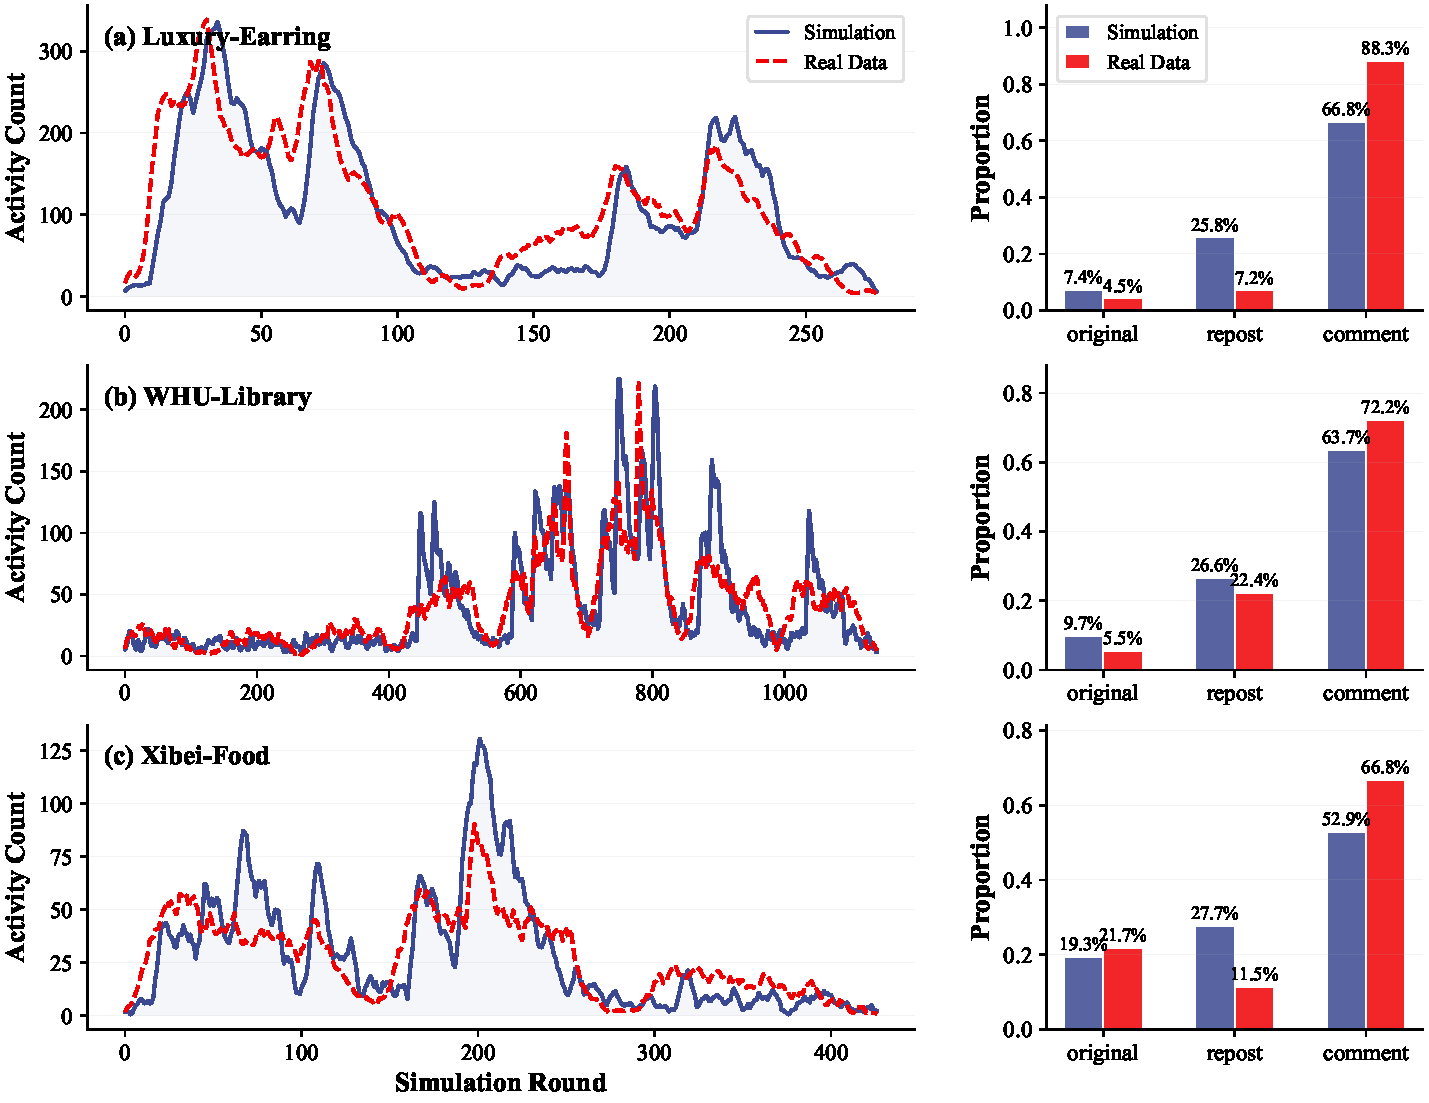
\includegraphics[width=\columnwidth]{fig_three_event_calibration.pdf}
\caption{三个事件的行为热度与分布校准结果。每行对应一个事件（(a)~天价耳环、(b)~武大图书馆、(c)~西贝预制菜），左侧为模拟与真实数据的活跃度时序对比，右侧为行为类型的比例分布对比。}
\label{fig:three_event_calibration}
\end{figure}

\end{document}

